% !TEX option = -shell-escape
% Important: The shell-escape flag is required for the Minted package.
% Please compile this document with 'pdflatex -shell-escape main.tex'.
% If you are using another IDE, you may be able to specify this in the
% options or to provide an option like '% !TEX option = -shell-escape'
% in this file, depending on your builder. See the README.md for more.

% Don't put any content in here.
% Don't even include content files by using \input or \inlcude.
% Put your content into components/text.tex or include it there using \input.
% You probably want to modify the following files:
%   components/info.tex             contains the author, title etc.
%   components/settings.tex         contains the packages and settings.
%   components/commands.tex         contains helpful custom commands.
%   components/glossary.tex         contains an explanation of the used terms.
%   components/acknowledgements.tex contains the acknowledgements.
%   components/quote.tex            contains a quote.
%   components/abstract.tex         contains the abstract of the document.
%   components/text.tex             includes the actual content of the document.
%   components/outline.tex          contains the outline.
%   components/preface.tex          contains the preface.
%   chapters/                       contains the main text.
%   bibliography/literature.bib     contains the BibTeX entries.
%   images/                         contains all your content-related images.
%
% You probably don't need to change anything in the following files:
%   components/cover.tex            formats the front cover of the document.
%   components/titlepage.tex        formats the title page of the document.
%   components/disclaimer.tex       formats the disclaimer page.
%   styles/                         contains style elements (e.g. logos).
%   main.tex                        contains the top-level code structure.
%   README.md                       contains information about this template.

\documentclass[11pt,
              a4paper,
              index=totoc,
              headsepline,
              footsepline,
              BCOR=12mm,
              DIV=13,
              oneside]{scrbook}

\usepackage[a4paper,includeall,bindingoffset=0cm,margin=3cm,hoffset=-0.5cm,
marginparsep=0cm,marginparwidth=0cm]{geometry}


% KOMA scrbook options:
%  index=totoc: include an entry for the index in the table of contents.
%  headsepline: use horizontal line under heading.
%  footsepline: use horizontal line above footer.
%  BCOR: binding correction (e.g.: BCOR=12mm)
%  DIV: Number of sheet sections (used for layout) (e.g.: DIV=13)

% !TEX root = ../main.tex
% Set here the title, authors and other stuff to be used for the cover
% This file is used by MAIN.TEX

% set title, authors and stuff for the cover
\def\university{Technical University of Munich}
\def\universityLogo{styles/tum_logo}
\def\program{Computer Vision Group\\TUM Department of Informatics}
\def\programLogo{styles/cse_logo}
\def\doctype{Bachelor's Thesis in Informatics}

\def\title{Physically constrained networks}
\def\titlegerman{Physikalisch bedingte Neuronale Netzwerke}
\def\author{Korbinian Abstreiter}
\def\examinerOne{Prof. Dr.-Ing. Laura Leal-Taixe}
\def\examinerTwo{Examiner two}
\def\assistantAdvisor{M.Sc. Patrick Dendorfer}
\def\date{July 15th, 2019}

\def\keywords{{keyword1}, {keyword2}, {keyword3}}

% The following are used for the PDF metadata, by default the same as above.
\def\metaTitle{\title}
\def\metaAuthor{\author}
\def\metaSubject{\doctype\ -\ \university}
\def\metaKeywords{\keywords}

% text to appear in the footer
\def\footertext{}


% !TEX root = ../main.tex
% Included by MAIN.TEX

%--------------------------------------------------
% Fonts and page setup
%--------------------------------------------------

\usepackage{booktabs}
\usepackage{amsmath}
\DeclareMathOperator*{\argmax}{argmax}
\DeclareMathOperator*{\argmin}{argmin}
\usepackage{amsthm}
\usepackage{graphicx}
%\usepackage{svg}
\usepackage{float}
\graphicspath{ {./images/} }
\usepackage{verbatimbox}

%\usepackage[]{epstopdf}
%\epstopdfsetup{outdir=./images/}

% Default font
\usepackage{palatino}

% Enable special PostScript fonts (optional)
% \usepackage{pifont}

% Manipulate the footer
\usepackage{scrpage2}
\usepackage{scrhack}
\pagestyle{scrheadings}

\automark[subsection]{section}
\renewcommand{\sectionmark}[1]{\markboth{\sectionmarkformat #1}{}}%
\renewcommand{\subsectionmark}[1]{\markright{#1}} %nur Titel ohne Nr.
\ihead{\leftmark}
\ohead{\rightmark}
\cfoot{\pagemark} 
\chead{}

%\ifoot[\footertext]{\footertext} % \footertext set in INFO.TEX

% Set the font for the section headings
\renewcommand{\sectfont}{\normalfont \bfseries}

% Conditional commands in LaTeX documents, used for the \clearemptydoublepage.
\usepackage{ifthen}

% Typeset text in multiple columns (optional)
% \usepackage{multicol}

% Rotation tools, including rotated full-page floats (optional)
\usepackage{rotating}


%--------------------------------------------------
% Document structure
%--------------------------------------------------

% Pro­duce hy­per­text links in the doc­u­ment (recommended)
\usepackage{hyperref}

% Create glossaries and lists of acronyms
% depending on how many packages were shipped with your TeX distribution,
% you might need to install xindy. On Linux: sudo apt install xindy
\usepackage[toc, xindy]{glossaries}

% Standard LaTeX package for creating indexes
\usepackage{makeidx}


%--------------------------------------------------
% Bibliography
%--------------------------------------------------

% Set the bibliography style (default: plain)
\bibliographystyle{plain}

% Special biblography package (nice to have)
% \usepackage{natbib}


%--------------------------------------------------
% Graphics and floats
%--------------------------------------------------

% Enhanced support for graphics (recommended)
%\usepackage{graphicx}
% Path to the figures directory (default: {figures/})
% Multiple entries are allowed, e.g. {{figures1/}{figures2/}}.
%\graphicspath{{./images/}}

% Improved interface for floating objects (optional)
%\usepackage{float}

% To use the subfigures (optional)
\usepackage{subcaption}


%--------------------------------------------------
% Mathematics
%--------------------------------------------------

% TeX fonts from the American Mathematical Society (recommended)
\usepackage{amsfonts}

% Some extra math symbols (optional)
% \usepackage{amssymb}

% Extended maths fonts for LaTeX (optional)
% \usepackage{yhmath}

% Provide math delimiters whose size can be computed automatically (optional)
% \usepackage{commath}


%--------------------------------------------------
% Source code and algorithms
%--------------------------------------------------

% Source code typesetting
% \usepackage{listings} % (optional - alternative)
\usepackage[newfloat]{minted} % (recommended)
% Set global Minted options
\setminted{linenos, autogobble, frame=lines, framesep=2mm}
% Inline C++ (optional)
\newcommand{\incpp}[1]{\mintinline{c++}{#1}}
\newenvironment{code}{\captionsetup{type=listing}}{}
\SetupFloatingEnvironment{listing}{name=Source Code}

% Typeset algorithms - pseudocode (optional)
% \usepackage{algorithmicx}
% \usepackage{algpseudocode}
% Normal arrow comments
% \algrenewcommand{\algorithmiccomment}[1]{\hfill$\rightarrow$ #1}


%--------------------------------------------------
% Tables
%--------------------------------------------------

% Tables (optional)
\usepackage{tabu}

% Add color to LaTeX tables (optional)
% \usepackage{colortbl}

% Create tabular cells spanning multiple rows (optional)
% \usepackage{multirow}


%--------------------------------------------------
% Color
%--------------------------------------------------

% Use colors
\usepackage[dvipsnames]{xcolor}

% You may find all the pre-defined colors in
% https://en.wikibooks.org/wiki/LaTeX/Colors#Predefined_colors

% Custom colors
\definecolor{Pantone300C}{HTML}{0065BD} % TUM primary blue
\definecolor{Pantone301}{HTML}{005293}  % TUM secondary light blue
\definecolor{Pantone540}{HTML}{003359}  % TUM secondary dark blue
\definecolor{DarkGray}{HTML}{333333}    % TUM secondary dark gray
\definecolor{MediumGray}{HTML}{808080}  % TUM secondary medium gray
\definecolor{LightGray}{HTML}{CCCCC6}   % TUM secondary light gray
\definecolor{Pantone7527}{HTML}{DAD7CB} % TUM accent gray
\definecolor{Pantone158}{HTML}{E37222}  % TUM accent orange
\definecolor{Pantone383}{HTML}{A2AD00}  % TUM accent green
\definecolor{Pantone283}{HTML}{98C6EA}  % TUM accent very light blue
\definecolor{Pantone542}{HTML}{64A0C8}  % TUM accent light blue

% Color for the hyperlinks (e.g. table of contents)
\def\colorLinks{Pantone300C}
% Color for the web links
\def\colorUrl{Pantone542}
% Color for the citations
\def\colorCitations{Pantone158}

%--------------------------------------------------
% PDF output
%--------------------------------------------------

% Adjust the color of the links
%\hypersetup{
%  linkcolor=\colorLinks,%
%  urlcolor=\colorUrl,%
%  citecolor=\colorCitations
%}
\hypersetup{
	linkcolor=black,%
	urlcolor=black,%
	citecolor=black
}

% Disable the coloring of the links when printing.
% Requires a compatible PDF reader.
\usepackage[ocgcolorlinks]{ocgx2}[2017/03/30]

% PDF Metadata
\hypersetup{
  pdftitle={\metaTitle},%
  pdfauthor={\metaAuthor},%
  pdfkeywords={\metaKeywords},%
  pdfsubject={\metaSubject}
}

% Create XMP Metadata (uses the values from hyperref)
\usepackage{hyperxmp}

% Make thumbnails (optional)
% \usepackage{thumbpdf}


%--------------------------------------------------
% Other settings
%--------------------------------------------------

% Define commands that appear not to eat spaces (optional)
\usepackage{xspace}


% !TEX root = ../main.tex
% Included by MAIN.TEX
% Please include your own cool commands here.
% Be only sure to comment it sufficiently so others can use it.

%-------------------------------------------------------------
%                      Own Commands
%-------------------------------------------------------------


%-------------------------------------------------------------
% math stuff -------------------------------------------------


% nice R, N, C
\newcommand{\nat}{\mathbb{N}}
\newcommand{\real}{\mathbb{R}}
\newcommand{\compl}{\mathbb{C}}

% norm
%\newcommand{\norm}[1]{\left\| #1 \right\|}

% un demi
\newcommand{\half}{\frac{1}{2}}

% parantheses
\newcommand{\parenth}[1]{ \left( #1 \right) }
\newcommand{\bracket}[1]{ \left[ #1 \right] }
\newcommand{\accolade}[1]{ \left\{ #1 \right\} }
%\newcommand{\angle}[1]{ \left\langle  #1 \right\rangle }

% partial derivative: %#1 function, #2 which variable
% simple / single line version
\newcommand{\pardevS}[2]{ \delta_{#1} f(#2) }

% fraction version
\newcommand{\pardevF}[2]{ \frac{\partial #1}{\partial #2} }

% render vectors: 3 and 4 dimensional
\newcommand{\veciii}[3]{\left[ \begin{array}[h]{c} #1 \\ #2 \\ #3	\end{array} \right]}
\newcommand{\veciv}[4]{\left[ \begin{array}[h]{c} #1 \\ #2 \\ #3 \\ #4	\end{array} \right]}

% render matrices: 3  dimensional (arguments in row first order)
\newcommand{\matiii}[9]{\left[ \begin{array}[h]{ccc} #1 & #2 & #3 \\ #4 & #5 & #6 \\ #7 & #8 & #9	\end{array} \right]}


%-------------------------------------------------------------
%-------------------------------------------------------------


%-------------------------------------------------------------
% some abreviations ------------------------------------------
\newcommand{\Reg}{$^{\textregistered}$}
\newcommand{\reg}{$^{\textregistered}$ }
\newcommand{\Tm}{\texttrademark}
\newcommand{\tm}{\texttrademark~}
\newcommand {\bsl} {$\backslash$}

%-------------------------------------------------------------
%-------------------------------------------------------------


%-------------------------------------------------------------
% formating --------------------------------------------------

% Theorem & Co environments and counters
\newtheorem{theorem}{Theorem}[section]
\newtheorem{lemma}[theorem]{Lemma}
\newtheorem{corollary}[theorem]{Corollary}
\newtheorem{remark}[theorem]{Remark}
\newtheorem{definition}[theorem]{Definition}
\newtheorem{equat}[theorem]{Equation}
\newtheorem{example}[theorem]{Example}
%\newtheorem{algorithm}[theorem]{Algorithm}

% inserting figures
\newcommand{\insertfigure}[4]{ % Filename, Caption, Label, Width percent of textwidth
	\begin{figure}[htbp]
		\begin{center}
			\includegraphics[width=#4\textwidth]{#1}
		\end{center}
		\vspace{-0.4cm}
		\caption{#2}
		\label{#3}
	\end{figure}
}

% referecing figures

\newcommand{\refFigure}[1]{ %label
	figure \ref{#1}
}
\newcommand{\refChapter}[1]{ %label
	chapter \ref{#1}
}

\newcommand{\refSection}[1]{ %label
	section \ref{#1}
}

\newcommand{\refParagraph}[1]{ %label
	paragraph \ref{#1}
}

\newcommand{\refEquation}[1]{ %label
	equation \ref{#1}
}

\newcommand{\refTable}[1]{ %label
	table \ref{#1}
}

\newcommand{\rigidTransform}[2]
{
	${}^{#2}\!\mathbf{H}_{#1}$
}

% comment that appears on the border - very practical !!!
\newcommand{\comment}[1]{\marginpar{\raggedright \noindent \footnotesize {\textsl{#1}} }}

% page clearing
\newcommand{\clearemptydoublepage}{%
  \ifthenelse{\boolean{@twoside}}{\newpage{\pagestyle{empty}\cleardoublepage}}%
  {\clearpage}}

%-------------------------------------------------------------
%-------------------------------------------------------------

\newcommand{\etAl}{\emph{et al.}\mbox{ }}


% !TEX root = ../main.tex
\newglossaryentry{computer}
{
  name=computer,
  description={is a programmable machine that receives input,
               stores and manipulates data, and provides
               output in a useful format}
}

\newglossaryentry{poc}
{
  name={proof of concept},
  description={}
  }
\newglossaryentry{ui}
{
  name={user interface},
  description={}
  }
\newglossaryentry{ai}
{
  name={arithmetic intensity},
  description={a measure of floating-point operations (FLOPs)
              \hyphenation{per-formed} performed by a \hyphenation{gi-ven} given code or code section relative
              to the amount of memory accesses (Bytes) that are required
               to support those operations\cite{AI}}
  }

\newglossaryentry{speed-up}
{
  name={speed-up},
  description={the factor of temporal acceleration a program
  exhibits when additional computational resources are dedicated to it's execution.}
}

\newglossaryentry{directive pragmas}
{
  name={directive pragma},
  description={a computer programming language construct that specifies how a compiler
  should process input data} % sourced from wikipedia
}


\newglossaryentry{rc}{%SOURCE: wikipedia
name={race condition},
description={A race condition or race hazard is the behavior of an electronic,
 software, or other system where the output is dependent on the sequence or
 timing of other uncontrollable events. It becomes a bug when events do not
 happen in the order the programmer intended. The term originates with the idea
 of two signals racing each other to influence the output first.}
}
\newglossaryentry{dd}{
name={data dependencies},
description={}
}
\newglossaryentry{sisd}{
name={single instruction single data},
description={}
}
\newglossaryentry{simt}{
name={single instruction multiple threads},
description={}
}

\newglossaryentry{simd}{
name={single instruction multiple data},
description={}
}
\newglossaryentry{gp}{%SOURCE: wikipedia
name={Gaussian Plane},
description={The two dimensional plane of complex numbers.}
}
\newglossaryentry{CURAND}{
name={CURAND},
description={
The CURAND library provides facilities that focus on the simple and efficient
generation of high-quality pseudorandom and quasirandom numbers.\cite{cuRAND}
}
}

\newacronym[longplural={partial differential equations}]{PDE}{PDE}{partial differential equations}
\newacronym{mpi}{MPI}{Message Passing Interface}

\newacronym[longplural={Random Walks on Spheres}]{RWoS}{RWoS}{Random Walk on Spheres}

\newacronym[longplural={graphical processing units}]{GPU}{GPU}{graphical processing unit}

\newacronym[longplural={central processing units}]{CPU}{CPU}{central processing unit}
\newacronym{hpc}{HPC}{high performance computing}

\newacronym[longplural={arithmetic logic units}]{ALU}{ALU}{arithmetic logic unit}

\newacronym[longplural={streaming multi-processors}]{SM}{SM}{streaming multi-processor}

\newacronym[longplural={boundary value problems}]{BVP}{BVP}{boundary value problem}
\newacronym[longplural={general purpose graphical processing units}]{GPGPU}{GPGPU}{general purpose graphical processing units}
\newacronym{CUDA}{CUDA}{compute unified device architecture}
\newacronym{RAM}{RAM}{random access memory}
\newacronym{SRAM}{SRAM}{static random access memory}
\newacronym{DRAM}{DRAM}{dynamic random access memory}
\newacronym{I/O}{I/O}{input/output}
\newacronym{PTX}{PTX}{Parallel Thread eXecution}
\newacronym{jit}{JIT}{just in time}


\makeglossary

\begin{document}

 \frontmatter

 % !TEX root = ../main.tex
% The front cover.
% Included by MAIN.TEX

%--------------------------------------------------
% The Front Cover
%--------------------------------------------------

% correct BCOR - undo at the end !!!
\def\bcorcor{0.15cm}
\addtolength{\hoffset}{\bcorcor}

\thispagestyle{empty}

\vspace{4cm}
\begin{center}
	\includegraphics[width=4cm]{\universityLogo}\\
	\vspace{5mm}
	\huge \program \\
	\vspace{0.5cm}
	\large \university
\end{center}

\vspace{20mm}
\begin{center}
	{\Large \doctype}\\
	\vspace{20mm}
	{\huge \textbf \title}\\
	\vspace{15mm}
	{\LARGE  \author}\\
	\vspace{\fill}
\end{center}

 \clearpage

 % !TEX root = ../main.tex
% The titlepage.
% Included by MAIN.TEX


%--------------------------------------------------
% The title page
%--------------------------------------------------

% correct BCOR - undo at the end !!!
\def\bcorcor{0.15cm}
\addtolength{\hoffset}{\bcorcor}

\thispagestyle{empty}

\vspace{4cm}
\begin{center}
    \includegraphics[width=4cm]{\universityLogo}\\
    \vspace{5mm}
    \huge \university\\
    \vspace{0.5cm}
    \Large \program \\
\end{center}

\vspace{10mm}
\begin{center}
    {\Large \doctype}\\
    \vspace{10mm}
    {\LARGE \title}\\
    \vspace{10mm}
    {\textit{\LARGE \titlegerman}}\\
	\vspace{10mm}
	
    \begin{tabular}{ll}
      \Large Author:                        & \Large \author \\[2mm]
      \Large Supervisor:& \Large \examinerOne\\[2mm]
      %\Large 2\textsuperscript{nd} examiner:& \Large \examinerTwo \\[2mm]
      \Large Advisor:             & \Large \assistantAdvisor \\[2mm]
      \Large Submission date:               & \Large \date
    \end{tabular}

    \vspace{\fill}
\end{center}

% undo BCOR correction
\addtolength{\hoffset}{\bcorcor}

 \clearpage

 % !TEX root = ../main.tex

\thispagestyle{empty}
\vspace*{0.8\textheight}
\noindent
I confirm that this bachelor's thesis is my own work and I have documented all sources and material used.

\vspace{15mm}
\noindent
\date \hspace{5cm} \author
\clearpage

% \clearpage

% % !TEX root = ../main.tex
\clearemptydoublepage
\phantomsection
\addcontentsline{toc}{chapter}{Acknowledgements}

\vspace*{2cm}

\begin{center}
{\Large \textbf{Acknowledgments}}
\end{center}

\vspace{1cm}

\begin{center}
If someone helped you or supported you through your studies, this page is a
good place to tell them how thankful you are.
\end{center}


%  \clearpage
\phantomsection

\begin{center}
\vspace*{11cm}
\textit{"People sometimes ask me if it is a sin in the Church of Emacs to use vi.
	Using a free version of vi is not a sin; it is a penance. So happy hacking"}
\end{center}
\par
\hspace*{7cm}
\textit{-Richard Stallman}


 % !TEX root = ../main.tex
% The abstract.
% Included by MAIN.TEX


%\phantomsection
%\addcontentsline{toc}{chapter}{Abstract}

\vspace*{2cm}
\begin{center}
{\Large \textbf{Abstract}}
\end{center}
\vspace{1cm}


Due to the rise of deep learning models in recent years, they are nowadays applied in a wide range of different tasks. Previously, problems could only be solved by hand-crafted models, which had to be designed individually for each task. Such models are based on principles that scientists and mathematicians have discovered and experimentally validated over many years. However, it does not only require much more effort to create a hand-crafted model, but there is also a high number of problems that can not be solved analytically, including many examples of differential equations. In contrast, deep learning models can be applied whenever training data is available, even when theoretical knowledge is sparse. However, the biggest limitation of data-driven models is the limited amount of available data for real world applications. As a consequence, their predictions deviate from the correct values and often do not align with known scientific principles. This raises the question if we purely have to rely on data to learn underlying mathematical theories which we know of and assume to be true.


%They have replaced a variety of hand-crafted models, since data-driven models require significantly less effort to create. In contrast to hand-crafted models, where every aspect of the system has to be implemented manually, deep learning models utilise the same algorithms for learning all kinds of problems and thus only sufficient hyperparameters have to be found. Furthermore, deep learning models can be used even when theoretical knowledge is sparse. However, for the predictions of data-driven models to align with theoretical constraints, such as the laws of physics, large amounts of training data covering the whole domain space are required. This raises the question, whether we have to purely rely on data to learn the mathematical theories which scientists have found and experimentally validated over many years. \\


\indent In this thesis, we examine and experiment with different approaches to incorporate knowledge of physical constraints into deep learning models. In particular, we analyse the Penalty Method and Augmented Lagrangian Method. In addition, we inspect the results when projecting predictions according to physical constraints during training. The benefits of these approaches are validated on the task of predicting a rotation in two and three dimensions with the constraints on the determinant of the rotation matrix and the preservation of the norm. We confirm that the methods lead to higher overall performance even for small training datasets and produce more realistic predictions in regions where no or only few training data is available.


\tableofcontents
 \clearpage
 
 \pagenumbering{arabic}

% \mainmatter

 % !TEX root = ../main.tex
% Included by MAIN.TEX
% Put your content in here or include it by using \input (\include won't work)

\addtolength{\evensidemargin}{-12mm}

% !TEX root = ../main.tex
\label{section:introduction}
\section{Introduction}

In recent years, deep learning models have proven to perform well in a wide range of applications, many of which include working with real world data. For example, Neural Networks have successfully been applied to the task of modeling lake temperature \cite{DBLP:journals/corr/abs-1710-11431} and fluid dynamics \cite{DBLP:journals/corr/SinghMD16}. Traditionally, such behaviours have been simulated by hand-crafted models. They were designed in a way to align with physical principles, such as gravity, the conservation of energy, or Newton's laws. This leads to high precision and avoids the problem of generalization, since the theories are assumed to be true accross the whole domain space. Nevertheless, manually building models requires intense effort and domain knowledge, and their performance may suffer from flawed parameter estimates or theories. In contrast, deep learning models do not rely on the complex underlying system structure. They can simply learn the behaviour from previously observed data. Furthermore, the latter outperform hand-crafted models in speed and can be applied even when no scientific theories are known. However, this comes to the high cost of large amounts of training data that is required for data-driven models to create realistic predictions aligning with physical principles. In addition, the data needs to be spread accross the whole domain space, which is often not the case. A lack of data in one region will already lead to unrealistic model predictions in that area, since the deep learning model does not specifically learn the physical rules and can therefore not generalize well.\\
\indent This raises the question, whether we can combine the scientific knowledge and the power of deep learning models in order to achieve more realistic results. Instead of purely relying on data, we can actively train the network to align its predictions with known physical principles. This could improve generalization and help to decrease the amount of data required and to create more realistic predictions.\\


\subsection{Related work}
Previously to this work, researches have published various approaches to incorporate knowledge about physical principles into deep learning models. \\
TODO: List related work

\clearpage



% !TEX root = ../main.tex
\label{section:theoreticalBackground}
\section{Theoretical Background}
In this section, we begin with introducing the general problem of optimisation. This is followed by the formulation of constrained optimisation problems, for which we give a more detailed description of different solving approaches. In particular, we focus on the Penalty Method and the Augmented Lagrangian Method.
\subsection{Optimisation problems}
Optimisation problems can be found in almost every field and researchers have come up with numerous algorithms to efficiently solve such tasks. Formally, an optimisation problem can be described as 
\[\argmin_{x \in \mathbb{R}^n} f(x),\]
where $f\colon \mathbb{R}^n\to \mathbb{R}$ is a smooth function to be minimised and $n \in \mathbb{N}$ is the input dimension. The objective function always has a set of local and global optima, where the latter are the ones we try to find.\\
In \cite{NoceWrig06}, Nocedal et al. describe the main approach optimization algorithms take to solve this problem. Since there is no known method to analytically find the solutions that minimise the objective function in the general case, such algorithms start at a point $x_0 \in \mathbb{R}^n$ and generate a sequence $\{x_k\}_{k=0}^\infty$. They are usually designed to converge to a local minimum, but have no guarantee for approximating one of the global optima. The sequence is terminated once a sufficiently good approximation of the solution is found or when no more progress can be made. If no solution exists, meaning that no point minimises the objective function, the algorithm might not terminate, since for any iterate a point with a smaller objective value can be found. The core of the algorithms is the way they use information about $f$ at the points $x_0, x_1, ..., x_k$ to compute $x_{k+1}$. \\
\indent Nocedal et al. introduce two categories of optimisation algorithms: Line search and trust region strategies. The former first determines a line on which the next iterate is located, and then tries to find a point $x_{k+1}$ such that $f(x_{k+1}) < f(x_k)$. Finding such an iterate is much simpler than the original minimisation problem, since a search only has to be performed along one dimension. The direction is often chosen to be the negative gradient, since it offers the locally steepest decent. 
\\ \indent In contrast, trust region strategies approximate the behaviour of the objective function $f$ inside a trust region $T$ around $x_k$ using a simpler model function $m_k$. The model function is often computed using the first terms of the Taylor expansion, that is \[m_k(x_k + p) = f(x_k) + p^T\Delta f(x_k) + \frac{1}{2}p^T\Delta^2 f(x_k) p \text{, \indent where } x_k + p \in T.\] Since the Hessian $\Delta^2 f(x_k)$ of the objective function can be hard to compute or not accessable, it can also be replaced by an approximation. The iterate $x_{k+1}$ is then set to be the solution of the simpler problem $x_{k+1} = \underset{x \in T}{\argmin }  \,\,m_k(x)$.

\subsection{Constrained optimisation problems}
Constrained optimisation problems are optimisation problems for which a solution has to satisfy given constraints. Formally, they can be described as the following:\\
\begin{equation}
	\label{constrained_min_problem}
	\begin{aligned}
		& \underset{x \in \mathbb{R}^n}{\argmin}
		& & f(x) \\
		& \text{subject to}
		& & c_i(x) \geq 0, \; i \in \mathcal{I}.
	\end{aligned}
\end{equation}

As before, $f\colon \mathbb{R}^n\to \mathbb{R}$ is our objective function and $n \in \mathbb{N}$ is the input dimension, whereas $c_i\colon \mathbb{R}^n\to \mathbb{R}, i \in \mathcal{I}$ are the inequality constraints with $\mathcal{I}$ denoting the set of all indices of the inequality constraints. Both $f$ and all $c_i, i \in \mathcal{I}$ are assumed to be smooth. Further, we also assume that a solution for the given problem exists. We call any point where no constraint is violated \textit{feasable}. Thus the \textit{feasable set} is defined as follows:
\[ \mathcal{F} := \{x \in \mathbb{R}^n \,|\, c_i(x) \geq 0, i\in \mathcal{I} \} \]

\indent In contradiction to unconstrained optimisation, where every local minimum $x^*$ satisfies $\Delta f(x^*) = 0$ and $\Delta^2 f(x^*)$ being positive semidefinite, solutions $\overline{x}$ of the constrained minimisation problem can be located on the boundary of the feasable set and thus $\Delta f(\overline{x}) = 0$ does not necessarily hold \cite{NoceWrig06}. In order to resolve this issue, we introduce the Lagrangian Relaxation as given in \cite{Lemarechal:2000:LR:647776.734757}. The Lagrangian for the constrained optimisation problem \eqref{constrained_min_problem} is defined as follows:
\[ \mathcal{L}(x, \lambda) = f(x) - \sum_{i \in \mathcal{I}} \lambda_i c_i(x), \]
where $\lambda \geq 0$ is the vector of Lagrangian multipliers. First of all, minimising the Lagrangian Relaxation is much easier than solving the inital problem, since we can apply algorithms for unconstrained optimisation to the former problem. Furthermore, this approach not only adds a bias towards feasable solutions, but more importantly allows the gradient on the boundary of the feasable region to equal zero in the direction of the gradient of the constraint. This can be achieved when using the correct values for the Lagrangian multipliers due to the additional gradient of the constraints eliminating the gradient of the objective function $f$ in the respective direction. However, this already indicates that setting the Lagrangian multipliers correctly is critical. Further, we have to note that $\mathcal{L}(x, \lambda) \leq f(x)$ for $x \in \mathcal{F}$, thus the Lagrangian provides a lower bound for $f$ for all feasable points. As a consequence, we can obtain the sharpest possible lower bound by solving the Lagrangian Dual, that is, 
\[ \underset{\lambda}{\max}\,\, \underset{x}{\min}\,\, \mathcal{L}(x, \lambda). \]
However, according to Boyd et al. as claimed in \cite{Boyd:2004:CO:993483}, there usually is a duality gap between the solution of minimising the constrained problem and its Lagrangian Dual problem. For convex problems, the authors provide necessary and sufficient conditions for a duality gap of zero given that $f$ and $c_i, i \in \mathcal{I}$ are convex.\\
\indent Even though we have no guarantee to find the exact solution for problem \eqref{constrained_min_problem} by solving the Lagrangian Dual, we introduce some optimality conditions which are more thoroughly explained in \cite{NoceWrig06}. First, we define a set of indices of the active constraints, that is
\[ \mathcal{A}(x) = \{ i \in \mathcal{I} \,|\, c_i(x) = 0 \}. \]
We further define the \textit{linear independence constraint qualification} (LICQ). It holds if the gradients of the active constraints $\{ \Delta c_i(x^*), i \in \mathcal{A}(x^*) \}$ are linearly independent. This ensures that no gradient of an active constraint is zero.
\begin{theorem}[\textit{Karush-Kuhn-Tucker conditions - KKT}]$\,$\\
	\label{theorem:kkt}
Let $x^*$ be a solution of the constrained optimisation problem \eqref{constrained_min_problem} for which LICQ holds. Then there exists a Lagrange multiplier vector $\lambda^*$, such that
\begin{subequations}
	\label{eq:kkt}
	\begin{align}
	\Delta_x \mathcal{L}(x^*, \lambda^*) &= 0,\\
	c_i(x^*) &\geq 0, \qquad \forall i \in \mathcal{I},\\
	\lambda^*_i &\geq 0, \qquad \forall i \in \mathcal{I},\\
	\lambda^*_i  c_i(x^*) &= 0, \qquad \forall i \in \mathcal{I}.
	\end{align}
\end{subequations}
\end{theorem}

The proof to Theorem \ref{theorem:kkt} is quite complex and can be found in \cite{NoceWrig06}. However, this statement is powerful, since it implies that for the right Lagrangian multipliers $\lambda$, solutions of the constrained optimisation problem have a gradient of zero in the relaxed problem and can therefore be found by unconstrained optimisation solving methods. Moreover, it provides an optimality test for solutions that minimise the Lagrangian, since the KKT conditions \eqref{eq:kkt} are necessary conditions for solutions of problem \eqref{constrained_min_problem}.\\



%\begin{theorem}
%Let $C(x) = \underset{i \in \mathcal{I}}{\sum} min(c_i(x), 0)^2$ be a function to measure the constraint violation of a given solution $x$. Further, let $x^* $ be a solution to the problem 
%\begin{equation}
%\label{minmax_constrained_opt}
%x^* = \underset{x \in \mathbb{R}^n}{\argmin}\, \underset{\mu }{\max}\, f(x) + \mu C(x).
%\end{equation} Then $C(x^*) = 0$ and $x^*$ is a solution for \eqref{constrained_min_problem}.
%\end{theorem}
%\begin{proof}
%	Let $\overline{x}$ be a solution of \eqref{constrained_min_problem}. It follows that $C(\overline{x}) = 0$, since $\overline{x}$ satisfies all constraints.\\
%	Now assume $C(x^*) > 0$, then we have $f(\overline{x}) + \mu C(\overline{x}) = f(\overline{x}) < f(x^*) + \mu C(x^*)$ for $\mu > (f(\overline{x} - f(x^*)) / C(x^*)$, which would make $x^*$ not a solution of \eqref{minmax_constrained_opt}. Therefore $C(x^*) = 0$. Further, we claim that $x^*$ is a solution for \eqref{constrained_min_problem}: If that was not the case, then $f(\overline{x}) < f(x^*)$ would hold. But because of $C(\overline{x}) = C(x^*) = 0$, we would have $\underset{\mu }{\max}\, f(\overline{x}) + \mu C(\overline{x}) < \underset{\mu }{\max}\, f(x^*) + \mu C(x^*)$, in which case $x^*$ would not be a solution of \eqref{minmax_constrained_opt}.
%\end{proof}

\subsection{Solving strategies}
In the following, we present two strategies to solve constrained optimisation problems. We first discuss the Penalty Method and continue with the Augmented Lagrangian Method. Both methods are based on the previsouly introduced idea of Lagrangian Relaxation.
\subsubsection{Penalty Method}
The first approach we introduce is the Penalty Method. As the name suggests, we penalise constraint violations, thus favoring feasable solutions. In particular, the values of each violated constraint is added quatratically to the objective function. This leads to a bias towards the feasable region. In contrast to the Lagrangian Relaxation, where the Lagrangian multipliers weight the constraints linearly to eliminate the gradients at the boundary, the Penalty Method does not take constraints into account that are satisfied at all. On the one hand, this leads to the advantage of leaving values of $f$ in the feasable region unchanged, on the other hand, gradients of solutions on the boundary of the feasable region are not manipulated either, which means that even solutions of the constraint optimisation problem on the boundary can have a gradient other than zero and are therefore no local minima. This problem is tackled by solving a series of minimisation problems while increasing the weight of the constraint penalisation, such that the global optimum of the function including the penalty converges to the global optimum of the objective function. Formally, each of the minimisation problems is of the following form:
\[\argmin_{x \in \mathbb{R}^n} Q(x, \lambda_k), \qquad Q(x, \lambda) := f(x) + \lambda \sum_{i \in \mathcal{I}} (c_i^{-}(x))^2\]
where $\{\lambda_k\}_{k=1}^\infty$ is a monotonically increasing series of weights with $\lim_{k \to \infty} \lambda_k = \infty$ and $c_i^-(x) = \min(0, c_i(x))$. Intuitively, this means that only violated constraints are penalised and as the penalty weight $\lambda$ increases, feasable solutions are favoured even more with each iteration.\\
In the following, we prove that the Penalty Method converges to an optimal solution.
\begin{theorem}
	Let $x_k = \argmin_{x \in \mathbb{R}^n} Q(x, \lambda_k)$. Then every limit point $x^* = \lim_{k \to \infty} x_k$ is a solution of the constrained minimisation problem \eqref{constrained_min_problem}.
\end{theorem}
\begin{proof}
	The proof is based on the proof given in \cite{NoceWrig06} with some adaptations to fit our problem formulation.\\
	Let $\overline{x}$ be a solution of problem \eqref{constrained_min_problem}. Thus the following holds: \[ f(\overline{x}) \leq f(x), \qquad \forall x \in \mathcal{F}\]
	Since $x_k$ minimises $Q(x, \lambda_k)$, we have 
	\begin{equation}
	\label{eq:pnlty_ineq1}
	f(x_k) + \lambda_k \sum_{i \in \mathcal{I}} (c_i^{-}(x_k))^2 \leq 
	f(\overline{x}) + \lambda_k \sum_{i \in \mathcal{I}} (c_i^{-}(\overline{x}))^2 =
	f(\overline{x})
	\end{equation}
	From this expression, we can now optain an upper bound on the constraint values, that is
	\begin{equation}
	\label{eq:pnlty_ineq2}
	\sum_{i \in \mathcal{I}} (c_i^{-}(x_k))^2 \leq \frac{1}{\lambda_k} (f(\overline{x}) - f(x_k)).
	\end{equation}
	Let $x^*$ be a limit point of $\{x_k\}$, thus there exists an infinite subsequence $\mathcal{K}$ with $\underset{k \in \mathcal{K}}{\lim} x_k = x^*$. Then we can obtain the following by applying the limit on both sides of the inequality \eqref{eq:pnlty_ineq2}:
	\[ 
	\sum_{i \in \mathcal{I}} (c_i^{-}(x^*))^2 = 
	\underset{k \in \mathcal{K}}{\lim} \sum_{i \in \mathcal{I}} (c_i^{-}(x_k))^2 \leq
	\underset{k \in \mathcal{K}}{\lim} \frac{1}{\lambda_k} (f(\overline{x}) - f(x_k)) = 0,
	 \]
	 since $\lambda \to \infty$. This implies that all constraints are satisfied and we only need to show $f(x^*) \leq f(\overline{x})$, which follows from taking the limit $k \to \infty, k \in \mathcal{K}$ in inequality \eqref{eq:pnlty_ineq1}:
	 \[ f(x^*) \leq f(x^*) +  \underset{k \in \mathcal{K}}{\lim} \,\,\lambda_k \sum_{i \in \mathcal{I}} (c_i^{-}(x_k))^2 \leq f(\overline{x})\]
\end{proof}

In general, the Penalty Method allows us to solve the constrained optimisation problem using methods for unconstrained optimisation on a series of minimisation problems. However, despite the existence of an analytical proof, a numeric conversion to the optimum of the constrained optimisation problem is not guaranteed. As Nocedal et al. point out in \cite{NoceWrig06}, the reason for this is that gradient based solving methods suffer from ill-conditioning when applied to $Q(x, \lambda)$ with large values for $\lambda$, which can not be avoided when trying to converge to a minimising and feasable solution.

\subsubsection{Augmented Lagrangian Method}
In the following, we introduce the Augmented Lagrangian Method (ALM). It tackles the problem of ill-conditioning as it occurs in the Penalty Method by adding the linear constraint term of the Lagrangian Relaxation with explicit estimates of the Lagrangian multipliers. We explain the case of having only a set of equality constraints $c_i(x) = 0, i \in \mathcal{E}$, where $\mathcal{E}$ is the set of indices of the equality constraints. This means the problem to solve is given by 
\begin{equation}
\label{constrained_min_problem_eq}
\begin{aligned}
& \underset{x \in \mathbb{R}^n}{\argmin}
& & f(x) \\
& \text{subject to}
& & c_i(x) = 0, \; i \in \mathcal{E}.
\end{aligned}
\end{equation}
The general case including inequalities can be solved by introducing slack variables; the interested reader is referred to \cite{NoceWrig06}.
The Augmented Lagrangian Method tries to solve the constrained problem \eqref{constrained_min_problem_eq} by solving a series of minimsation problems of the form
\[x_k = \argmin_{x \in \mathbb{R}^n} \mathcal{L}_A(x, \lambda_k, \mu_k), \qquad \mathcal{L}_A(x, \lambda, \mu) := f(x) - \frac{1}{2}\sum_{i \in \mathcal{E}} \lambda_i \,c_i(x) + \mu \sum_{i \in \mathcal{E}} c_i^2(x),\]
where $\{\mu_k\}$ is an increasing series, and the Lagrangian multipliers are updated according to the formula
\begin{equation}
\lambda_i^{k+1} = \lambda_i^k - \mu_k\,c_i(x_k).
\label{eq:alm_update}
\end{equation}
Assuming that the Lagrangian multipliers converge, we can see that the constraint values are now much smaller than $\frac{1}{\mu_k}$, since 
\[ c_i(x_k) = -\frac{1}{\mu_k}(\lambda_i^{k+1} - \lambda_i^k), \qquad i\in \mathcal{E}. \]
This means that in order to decrease the constraint values to close to zero, we do not purely rely on increasing $\mu$, but also achieve smaller constraint violations due to the convergence of the Lagrangian multiplier estimates. This makes it possible to show that ALM converges without increasing $\mu$ to an extremely large value as it is required for the Penalty Method \cite{NoceWrig06}.


\subsection{Related work}
Previously to this work, researches have published various approaches to solve constrained optimisation problems using deep learning models. One intuitive method is the so-called Projected Gradient Descent (PGD). As the name indicates, it projects the current iterate $y_k$ to the closest feasable solution $x_k \in \mathcal{F}$. Thus in case of the Euclidean orthogonal projection, it solves the following problem in each iteration:
\[ x_k = \argmin_{x \in F} ||x - y_k||_2, \]
where $y_k$ is calculated according to Gradient Descent with learning rate $\eta$, that is, $y_{k+1} = x_k - \eta \Delta f(x_{k})$ \cite{Chen}. This idea was also mixed with the Adam optimiser to keep the benefits of tracking momentum and adaptive learning rates by Marquez-Neila et al. in \cite{DBLP:journals/corr/Marquez-NeilaSF17}. Even though this procedure assures that all iterates are feasable and it yields good results, projections are often hard to compute when solving constrained problems with nonlinear constraints. \\
\indent As an alternative, Frank and Wolfe proposed an algorithm referred to as Conditional Gradients or Frank-Wolfe Algorithm in \cite{doi:10.1002/nav.3800030109}. Starting from the current iterate $x_k$ and a learning rate $\eta$, $x_{k+1}$ is obtained as follows:
\begin{subequations}
	\label{eq:frankwolfe}
	\begin{align}
		s_k &= \argmax_{s \in \mathcal{F}} \langle s, -\Delta f(x_k) \rangle \label{frankwolfe1},\\
		x_{k+1} &= (1-\eta) x_k + \eta s_k,
	\end{align}
\end{subequations}
where $\langle \cdot, \cdot \rangle$ denotes the inner product.\\
This means that the direction is obtained by going towards the point in the feasable set which aligns with the negative gradient most. The algorithm was also extended to the stochastic setting by Reddi et al. in \cite{Reddi2016StochasticFM}. Moreover, it has already been successfully applied to Computer Vision tasks such as 3D human pose estimation from a single view in \cite{DBLP:journals/corr/abs-1803-06453}. Despite the fact that the Frank-Wolfe Algorithm is projection-free, the computation of $s_k$ as described in equation \eqref{frankwolfe1} can also be difficult to solve when applied to a constrained problem with nonlinear constraints. Therefore, we focus our work on methods which do not incorporate hard constraints, but instead add soft constraints to the problems to be optimised.


\clearpage



% !TEX root = ../main.tex
\label{section:experiment}
\section{Experiment}
\begin{figure}[H]
	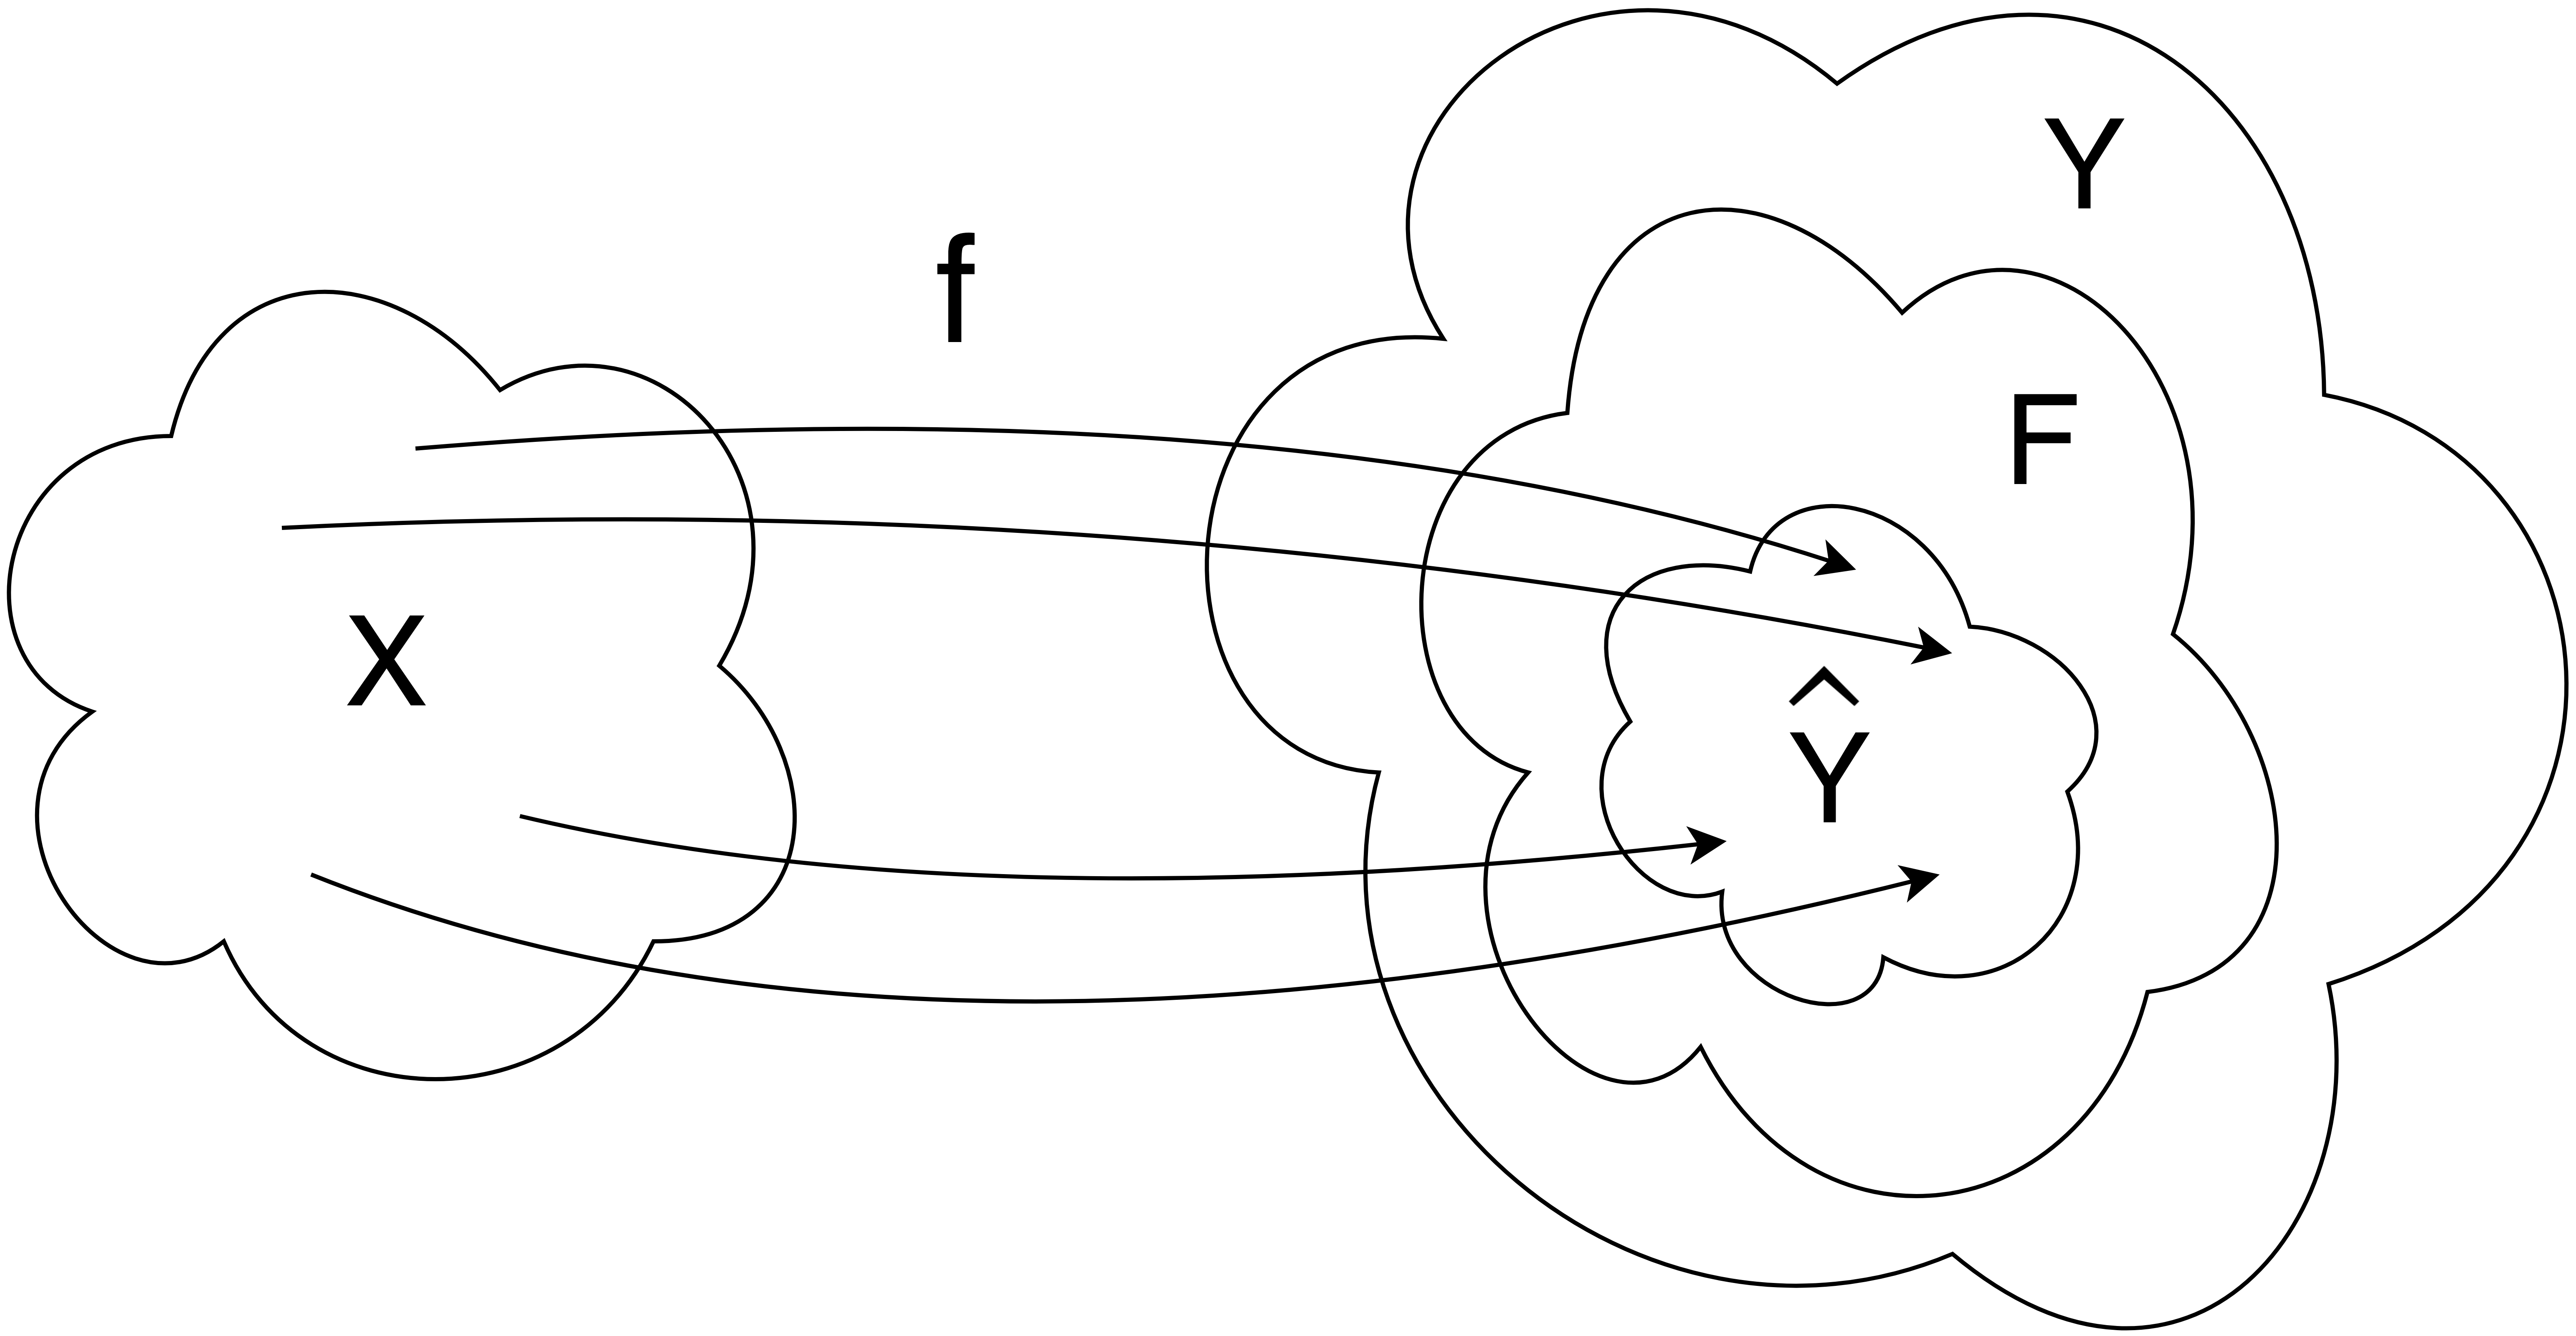
\includegraphics[width=\linewidth]{f_map}
	\caption{Visualisation of a function $f$ mapping from $X$ to $Y$. $F$ denotes the physically feasible set and $\hat{Y}$ the output values of $f$.}
	\label{fig:f_map}
\end{figure}
In general, a learning problem is to approximate a function $f: X \to \hat{Y}$ that maps given inputs of the domain $X$ to the corresponding output in the codomain $\hat{Y}$, as visualised in Figure \ref{fig:f_map}. Since we know that any output of $f$ satisfies all constraints, the set of outputs $\hat{Y}$ of $f$ is a subset of the feasible points $F$, meaning that $\hat{Y} \subseteq F$. However, when trying to learn the function $f: X \to \hat{Y}$, we usually do not know the set of ouputs $\hat{Y}$. Therefore, we start with the representation $f: X \to Y$, where $Y$ is a much larger space for which we know that $\hat{Y} \subseteq F \subseteq Y$. To give an example, we look at the following function:

\begin{equation}
\label{example_fn}
\begin{aligned}
g: &[0, \pi] \to [0, 1]\\
&x \mapsto \sin(x)
\end{aligned}
\end{equation}
Even though the function $g$ only maps values of the domain space $X = [0, \pi]$ to $\hat{Y} = [0, 1]$, feasible solutions contain all values between $-1$ and $1$, namely $F = [-1, 1]$, since we know that the function $\sin$ only outputs values in this range. Furthermore, when trying to learn $g$ without any prior knowledge about the function, we start by assuming that $g$ maps to the real numbers $Y = \mathbb{R}$.\\
\indent By incorporating physical constraints into the training process of deep learning models, we try to reduce the distance between the predictions $y_{pred} \in Y$ and the correct values $\hat{y}_{true} \in \hat{Y}$ by training the model to output values in or close to the feasable region $F$.\\
\indent Since it can be difficult to break down the effects utilising physical constraints has on a deep learning model, the previously introduced methods have to be applied to a simple, yet not trivial problem. Because we want to measure how well predictions align with the given constraints, we introduce the term \textit{realistic} to describe predictions with no or small constraint violations. By analysing the behaviour of our model, we aim to show that incorporating physical constraints contributes in the following ways:
\begin{itemize}
	\item Improve model performance,
	\item Create more realistic predictions,
	\item Decrease required amount of learning data.
\end{itemize}
A well fitting problem that satisfies both simplicity and the existence of physical constraints is provided by the task of learning a rotation. A rotation is a function that takes coordinates of a point together with rotation angles as input and outputs the coordinates of the rotated point.  The function can be described as a multiplication of a rotation matrix, which only depends on the rotation angle, and the point to be rotated. Rotations are invariant with respect to the L2-norm, meaning that the norm of the rotated point equals the norm of the input point. In addition, the determinant of the rotation matrix equals one. These two properties serve as physical constraints. Since the rotation problem satisfies the required characteristics, we use it to evaluate the previously introduced methods for incorporating physical constraints. The rotation problem itself is explained in more detail in the following section.

\subsection{Problem formulation}
In order to show the desired improvements, we apply the introduced methods to the rotation problem in both two and three dimensions. Formally, a rotation function maps a point and rotation angles to a target point:
\begin{equation}
\label{rot_fn}
\begin{aligned}
rot: \,\,&\mathbb{R}^{d} \times [- \pi, \pi] ^{d-1} \to \mathbb{R}^{d}\\
&(\vec{x}, \vec{\alpha}) \mapsto rot(\vec{x}, \vec{\alpha}) = \vec{y}
\end{aligned}
\end{equation}

, where $d$ is the dimension of the domain space. For example, the rotation in two dimension can be described in the following way:
\begin{equation}
\label{rot_fn_dim2}
\begin{aligned}
rot_{2D}: \,\,& \mathbb{R}^{2} \times [- \pi, \pi]  \to \mathbb{R}^{2}\\
&(\vec{x}, \vec{\alpha}) \mapsto rot_{2D}(\vec{x}, \vec{\alpha}) = R_{2D}(\vec{\alpha}) \,\vec{x}
\end{aligned}
\end{equation}
\[\text{where} \,\,R_{2D}(\alpha) = \begin{pmatrix} \cos(\alpha) & -\sin(\alpha) \\\sin(\alpha) & \cos(\alpha) \end{pmatrix}.\]
\indent For three dimensions, we will consecutively apply a rotation around the z-axis and the y-axis, both counterclockwise when looking towards the origin. This means that the rotation function maps the point $x$ and the rotation angles $\vec{\alpha} = \begin{pmatrix}
\alpha_1\\
\alpha_2
\end{pmatrix}$:
\begin{equation}
\label{rot_fn_dim3}
\begin{aligned}
rot_{3D}: \,\,& \mathbb{R}^{3} \times [- \pi, \pi]^2  \to \mathbb{R}^{3}\\
&(\vec{x}, \vec{\alpha}) \mapsto rot_{3D}(\vec{x}, \vec{\alpha}) = R_{3D}(\vec{\alpha})\,\vec{x} = R_{y}(\alpha_2) R_{z}(\alpha_1) \,\vec{x}
\end{aligned}
\end{equation}
where $R_{z}(\alpha) = \begin{pmatrix} \cos(\alpha) & -\sin(\alpha) & 0\\\sin(\alpha) & \cos(\alpha) & 0\\ 0 & 0 & 1\end{pmatrix}$
and $R_{y}(\alpha) = \begin{pmatrix} \cos(\alpha) & 0 & -\sin(\alpha)\\ 0 & 1 & 0\\\sin(\alpha) & 0 & \cos(\alpha)\end{pmatrix}$.\\
\\
\indent Regarding physical constraints, we know that the determinant of any rotation matrix equals one and thereby preserves the norm of any point. Therefore, we have the following two physical constraints for our experiment:

\begin{subequations}
\begin{equation}
\det (R(\vec{\alpha})) = 1, \qquad \forall \vec{\alpha} \in [-\pi, \pi]^d, \forall R \in \{R_{2D}, R_{3D}\}
\label{eq:constraint_det}
\end{equation}
\begin{equation}
||R(\vec{\alpha})\vec{x}||_2 = ||\vec{x}||_2, \qquad \forall \vec{\alpha} \in [-\pi, \pi]^d, \forall \vec{x} \in \mathbb{R}^d, \forall R \in \{R_{2D}, R_{3D}\}.
\label{eq:constraint_norm}
\end{equation}
\end{subequations}\\
The proofs for the determinant and norm constraint for two (resp., three) dimensions can be found in the Appendix in \eqref{proof:det_one} (resp., \eqref{proof:det_one_dim3}) and \eqref{proof:norm_preservation} (resp., \eqref{proof:norm_preservation_dim3}), respectively.

\subsection{Training the Deep Learning Model}
\indent Using a deep learning model, we can now learn the rotation function $rot$ as defined in equation \eqref{rot_fn} with the use of training data. Since the available training data is the biggest limitation for real life applications, we focus on improving the performance of neural networks using training datasets of limited sizes with prior knowledge about physical constraints. Therefore, we are mainly interested in the performance of our deep learning models with respect to the number of training datapoints. By comparing the model trained solely on the training data with the ones utilising the previously introduced methods, we try to show that incorporating the knowledge about physical principles increases both the performance and how well the predictions align with the physical constraints for limited amounts of training data. \\
\indent In the following, we explain technical details about the training dataset creation and the training process. For the remainder of this thesis, $N_{train}$ denotes the number of points included in our training dataset. The training data itself is denoted $X_{train}$. It contains $N_{train}$ elements of the set $\mathbb{R}^{d} \times [- \pi, \pi] ^{d-1}$. The corresponding correct target points are denoted $y_{train}$.\\
\indent The points to be rotated for the $2D$- and $3D$-Rotation are drawn uniformly from the unit circle and the unit sphere, respectively. The rotation angles are chosen uniformly from the set $[-\pi, \pi]^{d-1}$. Note that for three dimensions, this leads to a bias towards the poles, meaning that the target point is more likely to be either close to the original point or to the point located exactly on the opposite side of the sphere.\\
\indent When training a neural network to learn the rotation function, we solve the following minimisation problem:
\[\underset{\theta}\argmin \,\, \mathcal{L}(f_{\theta} (X_{train}), y_{train}), \]
where $f_\theta$ is the function represented by the model parameterised by $\theta$ and $\mathcal{L}$ is a loss function measuring the dissimilarity between the model predictions $f_{\theta} (X_{train})$ and the true target points $y_{train}$. From this point on, the model predictions $f_{\theta} (X_{train})$ for a fixed parameter set $\theta$ will be denoted by $\hat{y}$.
A commonly used loss function is the Mean Squared Error (MSE), which is calculated in the following way:
\begin{equation}
\label{eq:mse}
\mathcal{L}_{MSE}(\hat{y}, y) = \frac{1}{N}\sum_{n = 1}^{N} \frac{1}{d} \sum_{i = 1}^{d} (\hat{y}_{n\,i} - y_{n\,i})^2, \qquad \text{ where } y, \hat{y} \in \mathbb{R}^{N \times d}
\end{equation}

\indent All models will be trained using the MSE between the predictions and the target points. Minimising the MSE loss function fits well for our experiment, since it is closely related to the euclidian distance, except that distances are squared. This leads to high values for distant predictions and thus penalises higher variance of the errors of the predictions, which is desirable.\\ 

\subsection{Performance evaluation}
For the same reason as we chose the MSE Loss as the training loss, we also evaluate the performance of the introduced models and methods according to the MSE. Despite the MSE being a good measure for the distance between the predictions and the target point, it does not measure how well the predictions of the model align with the given physical constraints. In order to check how realistic the predictions are, we explicitely compare their norms and determinants.\\

\subsection{Network architectures}
\label{ssec:network_architectures}
In the following, we introduce three different model architectures parameterised with weights $\theta$ to learn the rotation function. The most important characteristics are depicted in Table \ref{table:model_archs}.
\begin{table}[H]
	\centering
	\caption{Model architectures for two dimensions. $\alpha$ is the rotation angle, $p_1$ and $p_2$ denote the coordinates of the input point and $\hat{y}$ is the predicted point. The operator \protect\includegraphics[height=8pt]{dotoperator} represents matrix-vector multiplication.}
	\label{table:model_archs}
	\begin{tabular}{ |c|c|c|c| } 
		\hline
		& Model 1 & Model 2 & Model 3 \\ 
		\hline
		\addvbuffer[0pt 1.4cm]{Structure} & 
		\addvbuffer[2pt 0pt]{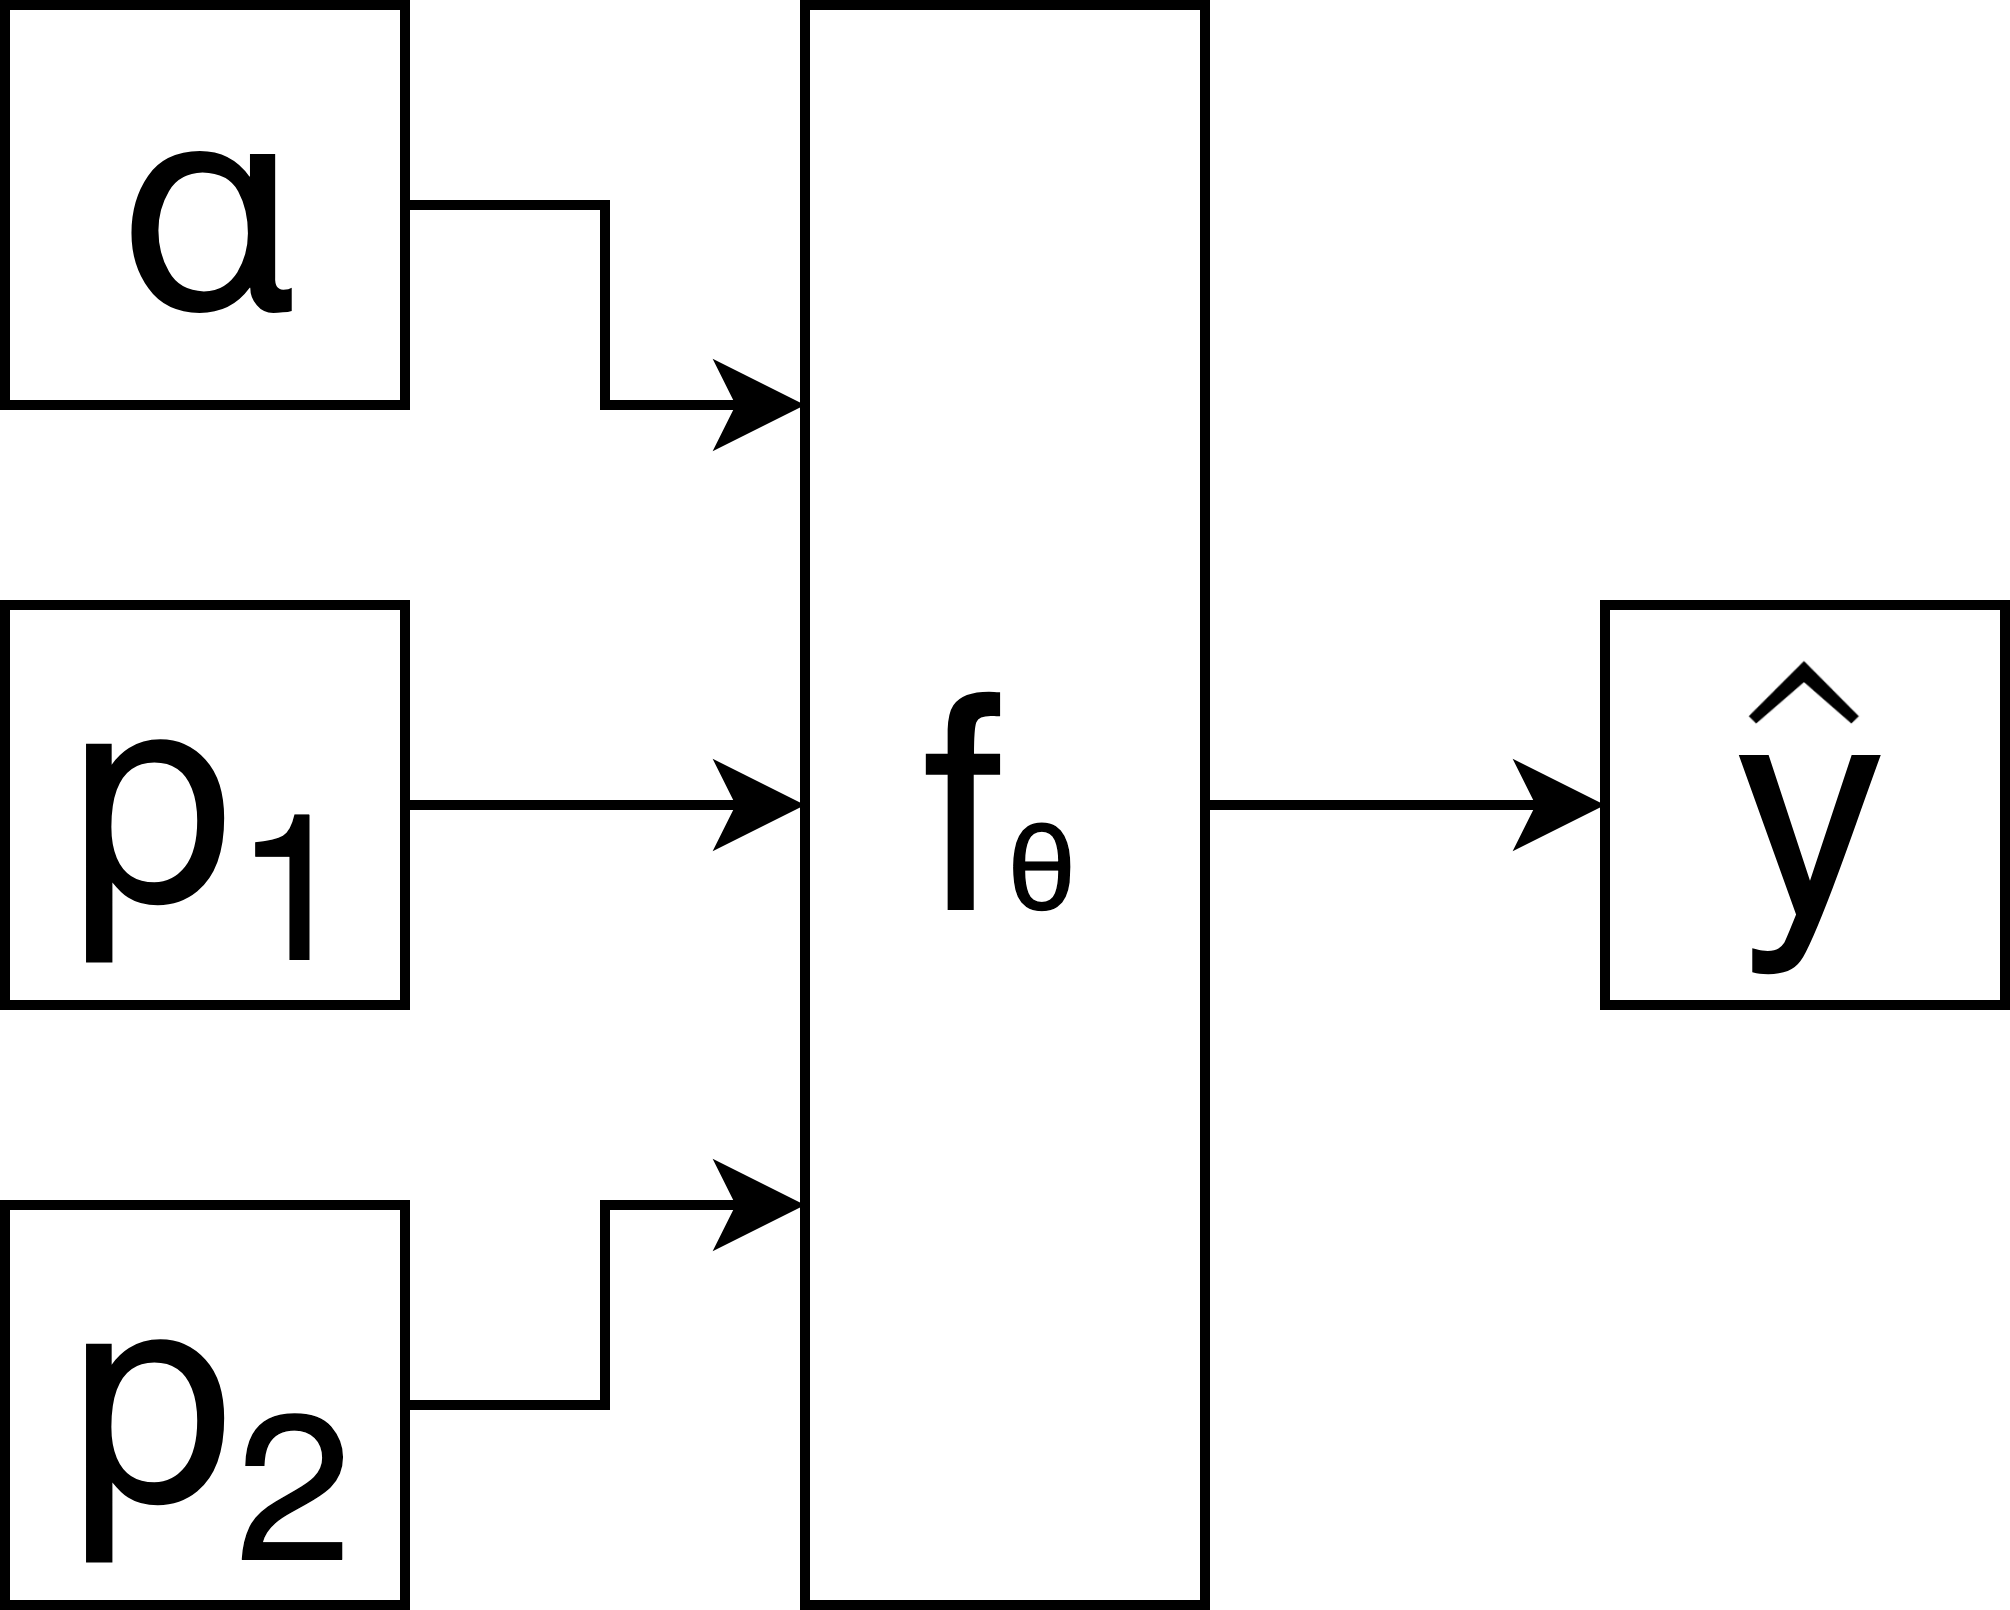
\includegraphics[height=2.5cm]{arch_model1}} & 
		\addvbuffer[2pt 0pt]{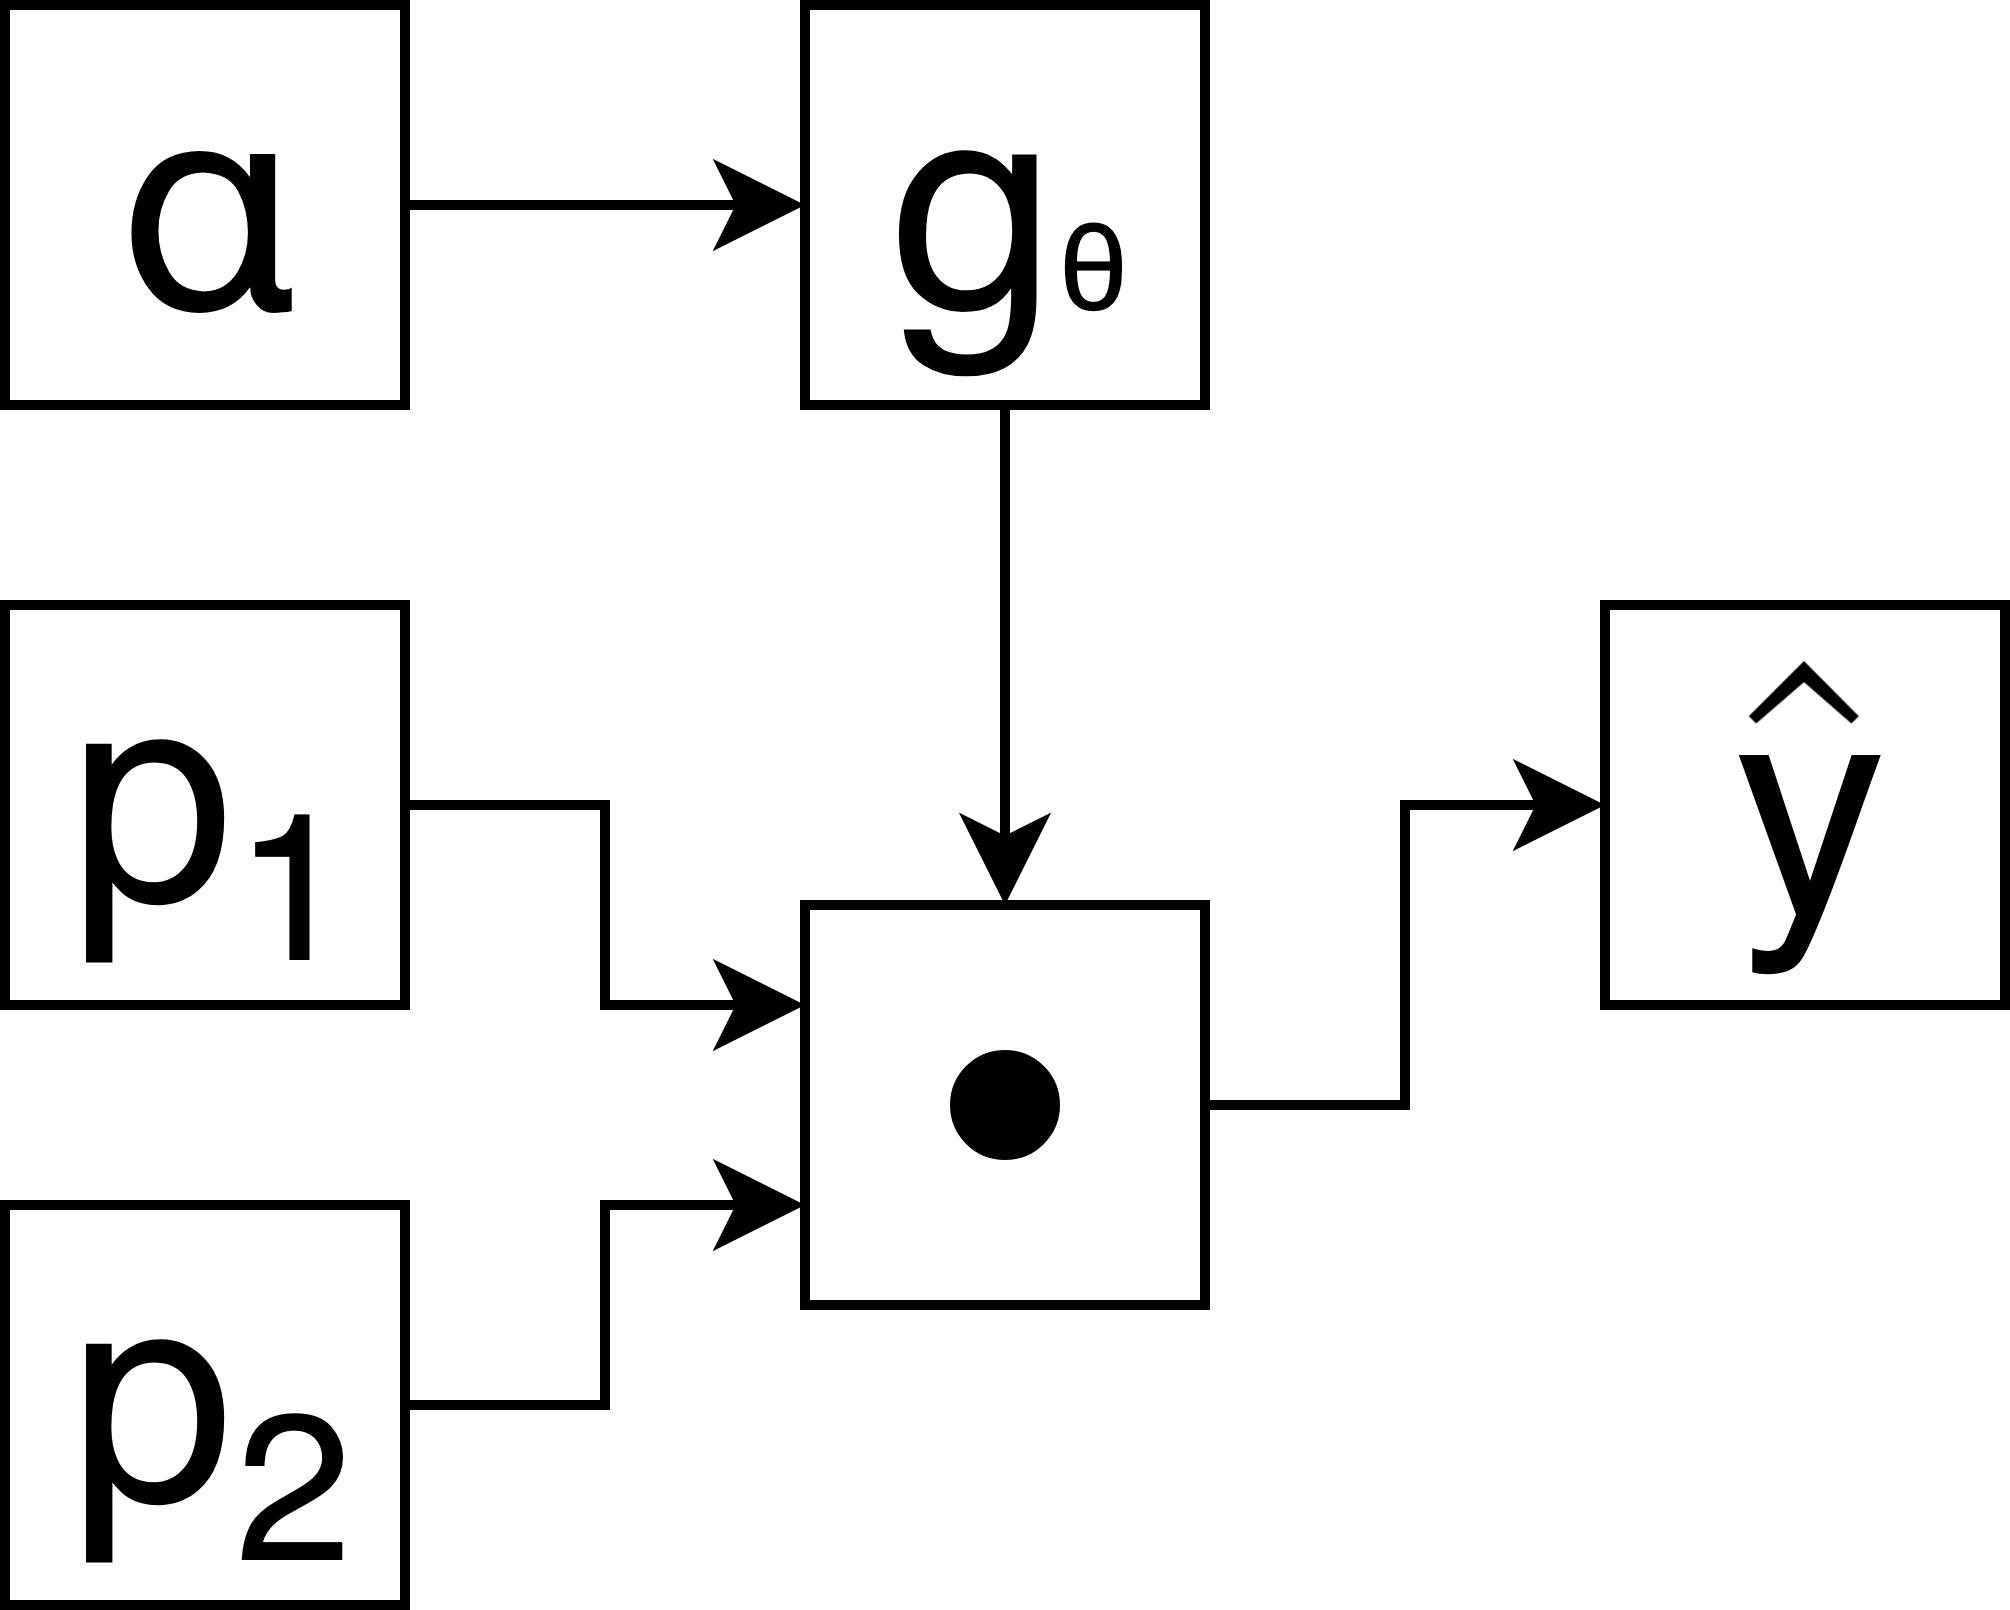
\includegraphics[height=2.5cm]{arch_model2}}  & 
		\addvbuffer[2pt 0pt]{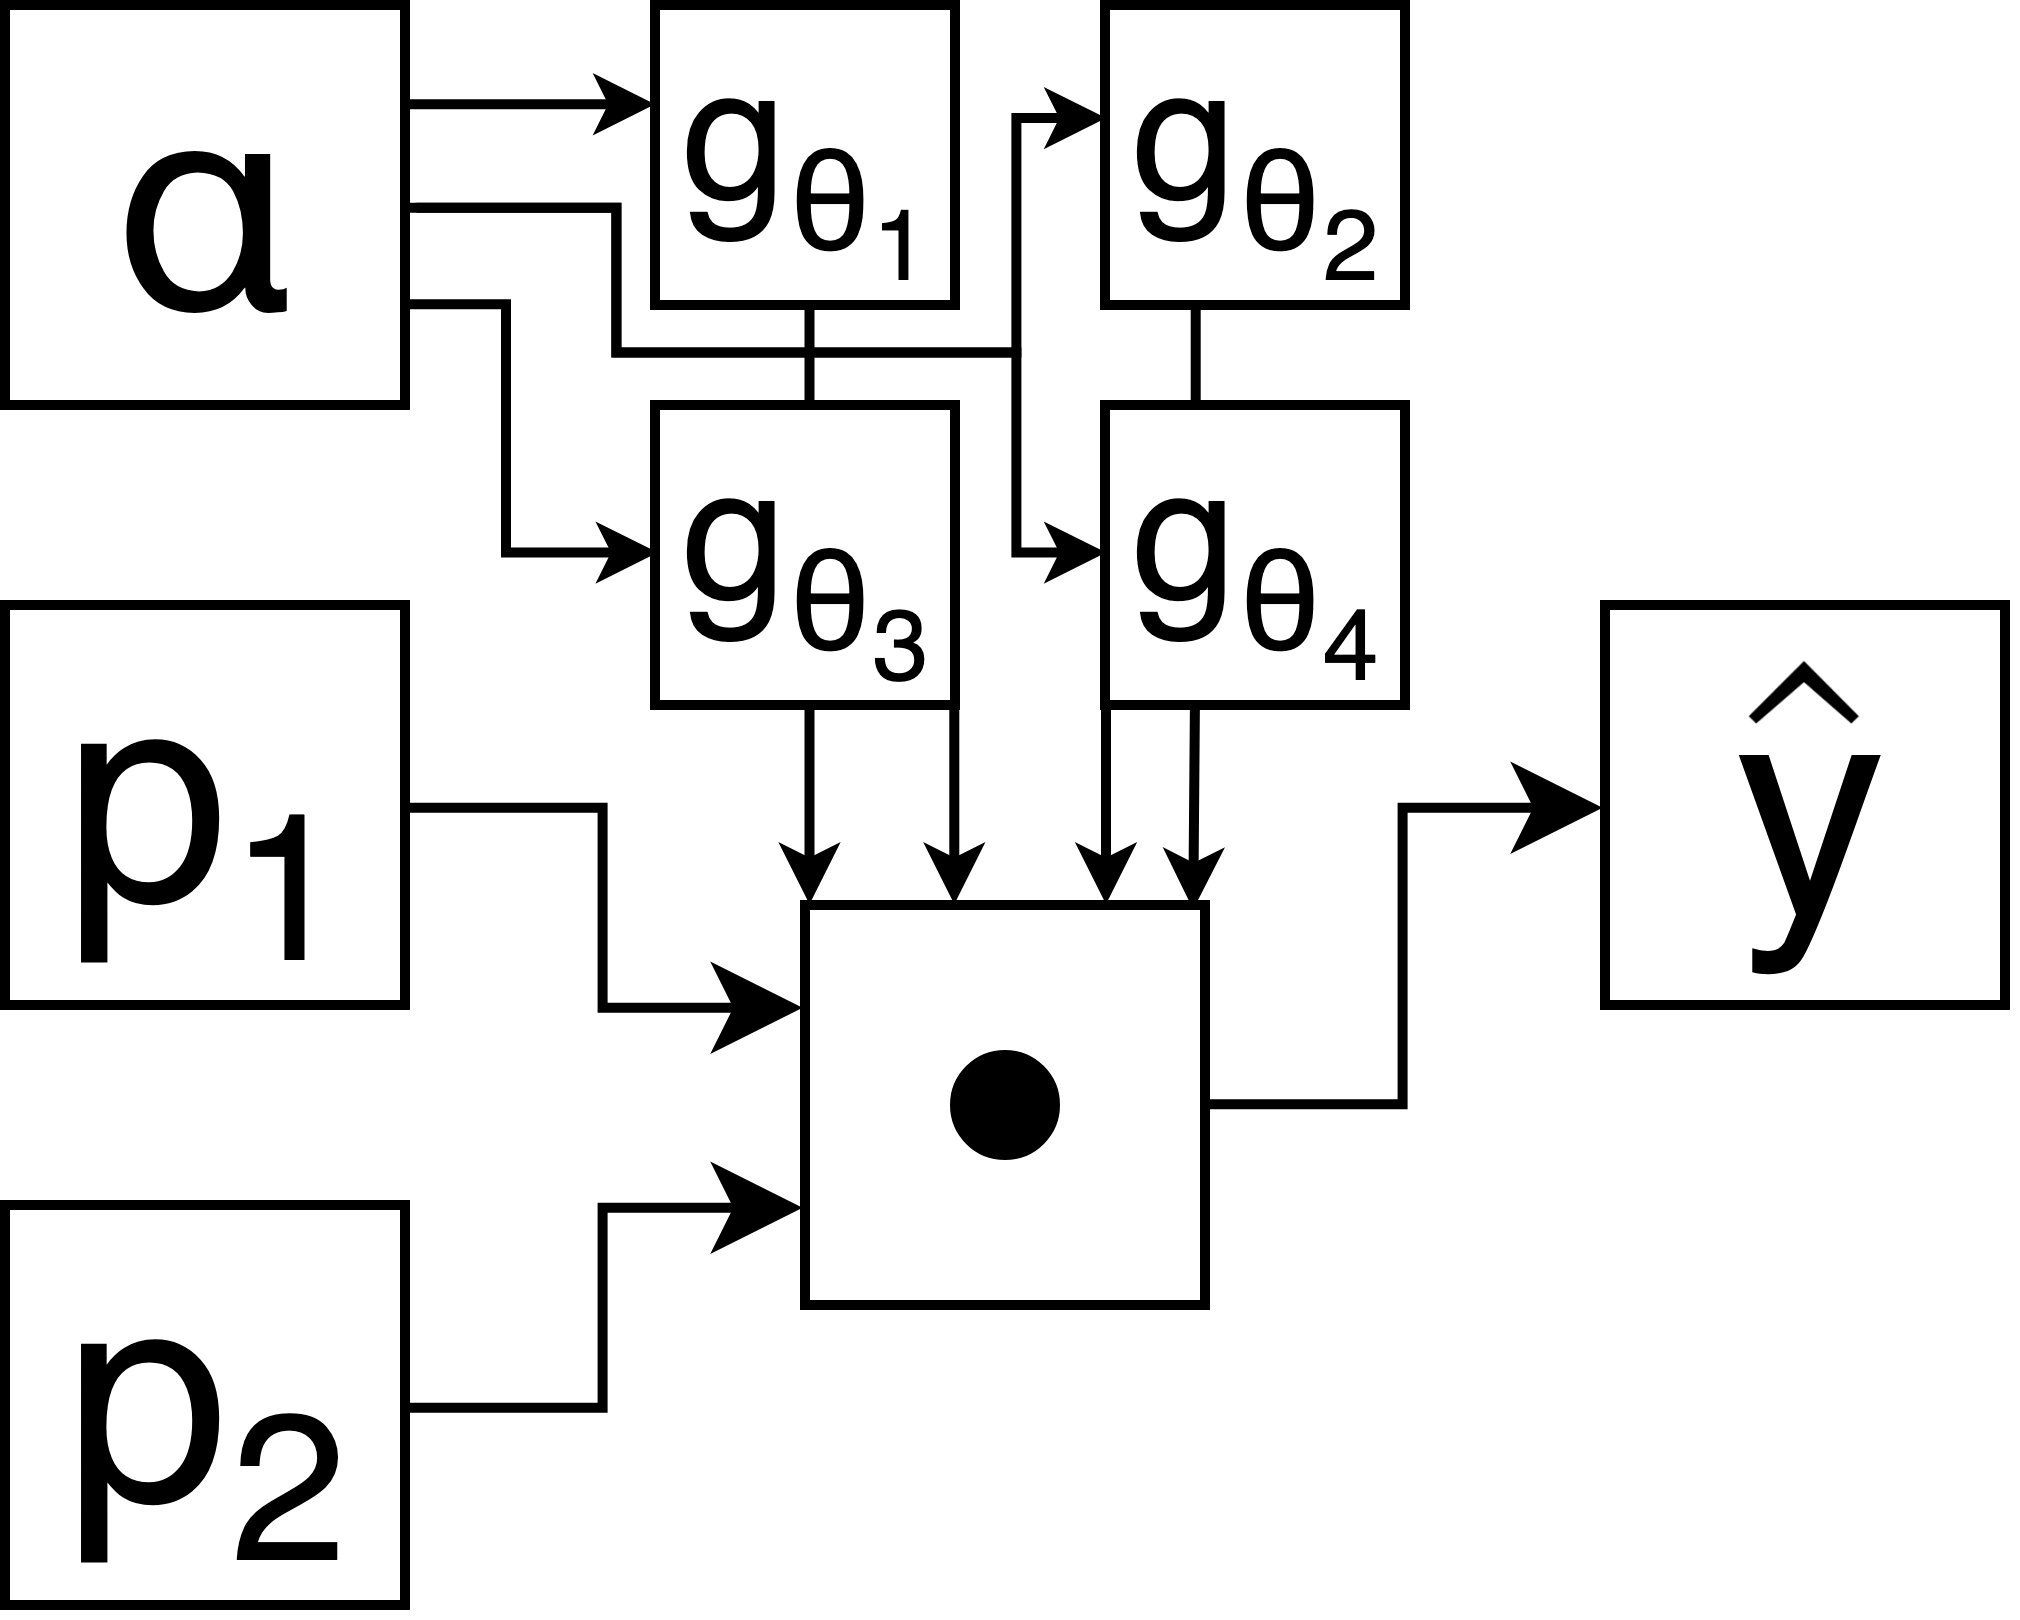
\includegraphics[height=2.5cm]{arch_model3}}  \\ 
		\hline
		\addvbuffer[3pt 0pt]{\shortstack{Network \\ function}} & 
		\addvbuffer[0pt 5pt]{$f_\theta: \mathbb{R}^3 \to \mathbb{R}^2$} & 
		\addvbuffer[0pt 5pt]{$g_\theta: \mathbb{R} \to \mathbb{R}^{2\times2}$} & 
		\addvbuffer[0pt 5pt]{$g_{\theta_i}: \mathbb{R} \to \mathbb{R}, i \in \{0, 1, 2, 3\}$} \\ 
		\hline
		Layer sizes & 
		$3 \to 16 \to 16 \to 16 \to 2$ &
		$1 \to 100 \to 4$ &
		$[1 \to 50 \to 1] \times 4$ \\
		\hline
		Activation & 
		Tanh &
		Sigmoid &
		Sigmoid \\
		\hline
		Parameters & 
		642 &
		604 &
		604 \\
		\hline
	\end{tabular}
\end{table}

\paragraph{Model 1:}The first model is a neural network directly approximating $f_\theta$. Thus it takes a point of dimension $d$ and angles of dimension $d-1$ as input and predicts a target point of dimension $d$. The network has three hidden layers with 16 nodes each. In each of the hidden layers, the activation function $\tanh$ is applied.\\

For \textbf{Model 2} and \textbf{Model 3}, we make use of the knowledge that a rotation is the result of multiplying a rotation matrix, which only depends on the angles, with the given point. Consequently, the networks of the next models represent the function $g_\theta: [-\pi, \pi]^{d-1} \to \mathbb{R}^{d \times d}$, which in turn is used to create the final predictions in the following way:
\begin{equation}
\label{eq:rot_pred}
\hat{y} = g_\theta(\alpha) \, p,
\end{equation}
where $\alpha \in [-\pi, \pi]^{d-1}$ is the rotation angle and $p \in \mathbb{R}^d$ the point to be rotated.

\paragraph{Model 2:} Based on this approach, the second model predicts the rotation matrix. In particular, it maps $d-1$ input angles to a matrix of size $d \times d$. This is done using one hidden layer of size 100 with Sigmoid activation function. 

\paragraph{Model 3:} Similar to the previous model, we also try to solve the problem using an independent neural network for each of the $d \times d$ matrix entries. Each of these networks maps the rotation angles of size $d-1$ to a single real number, which is interpreted as a single matrix entry. For these networks, we use one hidden layer of size 50 with the Sigmoid activation function.\\

\subsection{Hyperparameters}
All layers of the neural networks include bias and we do not apply dropout. In order to achieve undistorted comparisons of the models, they were designed to have between 600 and 650 parameters each for the two-dimensional problem. For all experiments, we decide to use the Adaptive Moment Estimator "Adam" as our optimiser, since it empirically appeared to perform well in practice and is favourable to other known adaptive learning-method algorithms \cite{DBLP:journals/corr/Ruder16}. Furthermore, we use a learning rate of $5\times 10^{-5}$ and train each model using $50\,000$ iterations. Both of these parameters are empirically estimated, a comparison of using different learning rates on Model 3 can be found in the appendix (\ref{fig:comp_lr_m3}). For all experiments, we use a batch size of 512 and shuffle the training set at the start of each epoch.

\subsection{Metrics}
In the following, we introduce different loss functions to measure the desired properties of the predictions. The choice of these loss functions is critical, since they determine the objective function which is minimised in the training process. In particular, the loss functions need to measure the predictions' accuracy and physical feasability.
\subsubsection{Accuracy}
As explained previously, the MSE Loss defined in equation \eqref{eq:mse} is a well fitting function to measure the accuracy of the predictions, since it is the sum of the square distances between the predictions and the corresponding target points. Hence, training on the MSE Loss aims to reduce this distance.
\subsubsection{Phyiscal feasability}
In order to train our models to learn the physical constraints, we introduce loss functions specifically designed to measure how realistic the model predictions are. In general, our physical loss functions map the predicted points and, if applicable, the predicted rotation matrix to a real number, which is interpreted as the violation of the physical constraints. Thus the physical loss functions are of the form
\[L_{PHY}: \mathbb{R}^d \times \mathbb{R}^{d \times d} \to \mathbb{R}. \]
\paragraph{Determinant constraint} 
In order to measure how well the predicted rotation matrices align with the constraint of the determinant being equal to one \eqref{eq:constraint_det}, we use the following function as our physical loss:
\[L_{DET}(\hat{y}, \hat{R}) = \frac{1}{N_{train}}\sum_{n = 1}^{N_{train}}(\det(\hat{R}_n) - 1)^2,\]
where $\hat{R}$ are the predicted rotation matrices computed by applying $g_\theta$ to each element of $X_{train}$. This can also be described as the MSE Loss between the vector of the predicted matrices' determinants and a vector of the same size filled with ones.
\paragraph{Norm constraint} 
In order to incorporate the constraint that the norm of any prediction needs to be one \eqref{eq:constraint_norm}, the following physical loss function is applied:
\[L_{NORM}(\hat{y}, \hat{R}) = \frac{1}{N_{train}}\sum_{n = 1}^{N_{train}}(||\hat{y}_n||_2 - 1)^2, \]
where $\hat{y}$ denotes the points predicted by the model. Similar to the Determinant loss, the Norm loss can be interpreted as the MSE Loss between the vector of the norms of the predictions and a vector of ones of the same size.

\subsection{Solving methods}
In this section, we will introduce the methods we apply to incorporate the physical loss functions into the models. As a baseline for comparisons, we train each model using solely the MSE Loss on the training data.

\subsubsection{Penalty Method}
The first and simplest version of the Penalty Method we apply is setting a fixed weight $\lambda > 0$ and solving a single minimisation problem, that is,

\[\underset{\theta}\argmin \,\, (\mathcal{L}_{MSE}(\hat{y}_\theta, y_{train}) + \lambda \cdot L_{PHY}(\hat{y}_\theta, g_\theta(X_{train}))).\]

In addition, we also solve a series of minimisation problems of the type above with exponentially increasing $\lambda$, but using the solution of the last iteration as a warm start for the next one. In particular, we introduce a multiplier $\mu > 1$ such that the weight of the physical loss in the i-th iteration is given by $\lambda_i = \mu^i \, \lambda_0$. Each minimisation is stopped as soon as the norm of the gradient is below a certain threshold.

\subsubsection{Augmented Lagrangian Method}
\label{exp:alm}
As we do for the Penalty Method, we also apply two different versions of the Augmented Lagrangian Method. Both versions minimise a fixed number of problems and update the weights of the linear constraint terms according to rule \eqref{eq:alm_update}. However, the first one only computes a fixed number of epochs with a constant weight $\lambda$ for the physical loss for each minimisation problem.\\
\indent The second version was suggested by Bertsekas in \cite{Yurkiewicz1985ConstrainedOA}. In addition to increasing the weight of the squared constraint term, he proposes to stop the minimisation of the k-th problem as soon as the norm of the gradient is smaller than a threshold $\tau_k$ computed according to the following equation:
\[\tau_k = \min(\epsilon_k, \gamma_k ||c(x_k)||_2), \]
where $\{\epsilon_k\}$ and $\{\gamma_k \}$ are two sequences decreasing to 0 and $c(x_k)$ is the value of the constraint violation at the current solution. In our experiment, $c(x_k)$ is the difference of the norms / determinants of the predicted points / rotation matrices and one. Intuitively, this approach spends more ressources on minimising a problem if the predictions of the current solution already align well with the physical constraints and otherwise focuses on learning the constraints first.

\subsubsection{Physical Projection}
\label{sec:phys_proj}
As a third approach, we apply the Physical Projection. In particular, each prediction in the training process is projected to the closest feasable prediction. When applying it to the norm loss, we divide the predicted point $\hat{y}$ by its norm and thus get a prediction $\hat{y}'$ located on the unit circle or unit sphere. Formally, predictions are calculated the following way:
\begin{equation}
\hat{y}' = \frac{\hat{y}}{||\hat{y}||_2}.
\end{equation}

For the determinant, we only divide the matrix by the $d$-th root of the determinant if the latter is positive, otherwise we do not change the matrix. Therefore any predicted rotation matrix with a positive determinant is projected to a new matrix with a determinant of one. Formally, we apply the following function to each predicted matrix $\hat{R}_n$:
\begin{equation}
\hat{R}_n' = \begin{cases} \frac{\hat{R}_n}{\sqrt[d]{\det(\hat{R}_n)}}, \qquad \text{if} \det(\hat{R}_n) > 0 \\ \hat{R}_n, \qquad \qquad \,\,\,\,\text{else} \end{cases}, \qquad n = 1, ..., N_{train}.
\label{eq:norm_det}
\end{equation}

Since matrices with negative determinants are far away from the true rotation matrix, they should not occur often or if so, be corrected by solely training on the MSE-Loss for the prediction and the target point. 

\subsection{Statistical measurements}
Each experiment will be tested on 20 different seeds used to generate the training data, with a few exceptions due to time limitations. If not otherwise specified, we compare the performance of the models according to the mean of the MSEs of the individual runs. We prefer the mean over the median, because we are also interested in the performance of outliers that lead to poor results. The test set on which each model's performance is calculated consinsts of 4096 data points sampled in the same manner as the training dataset.\\








\clearpage



% !TEX root = ../main.tex
\label{section:results}
\section{Results}

In this section, we compare the performance of the previously introduced models and methods and illustrate the results. They provide insight on the effects of incorporating knowledge about physical constraints and some limitations.

\subsection{Model architecture}
As described in the section \ref{ssec:network_architectures}, we first compare the three introduced network architectures. The performance of the models is displayed in Figure \ref{fig:models}.
\begin{figure}[ht]
	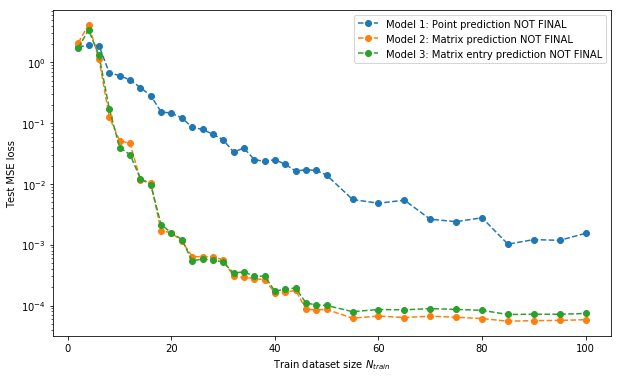
\includegraphics[width=\linewidth]{models}
	\caption{Different model architectures}
	\label{fig:models}
\end{figure}
We can see that while the difference between the behaviours of Model 2 and 3 is quite small, both of them perform significantly better than Model 1. Even when trained on 90 data points, Model 1 only achieves an error of $8\times 10^{-3}$, whereas Model 2 and 3 achieve a lower value of $2.7\times 10^{-3}$ with only 20 data points. This aligns with our expectations, since the latter two models already make use of the knowledge that a rotation can be represented as the multiplication of the point with a matrix that only depends on the rotation angle. Even though both matrix models perform well and almost the same for 20 and 30 data points, Model 2 finds a slightly better solution for most other amounts of training data. For example, with 10 data points, Model 2 achieves an error of $8.2\times 10^{-2}$, which is $41\%$ less than the performance of Model 3, which only reaches $1.4\times 10^{-1}$.\\
\indent In order to be able to extract the true effects of the methods we apply, all of the following experiments use one of the well performing models, which we choose to be Model 2. Since it already reaches a Test MSE Loss of less than $3\times10^{-3}$ with 20 training data points and still performs poorly with only 10 points, the majority of the following analysis focuses on the interesting region of 10 to 20 as the size of the training dataset. In order to make sure that the improvements of the following methods utilising the physical constraints are not due to the regularisation they entail, we checked that L2-Regularization has no significant or consistent positive impact. The results can be looked up in the appendix in Figure \ref{fig:reg_weights}.

\subsection{Penalty method}
\subsubsection{Fixed physical loss weight}
First, we apply the Penalty Method using a fixed weight $\lambda$ for the determinant physical loss $\mathcal{L}_{DET}$ and therefore only solve a single minimisation problem during the training process. The results obtained by this method performing 50000 epochs on the 2D-Rotation problem are shown in Figure \ref{fig:pnlty_det}.

\begin{figure}[ht]
	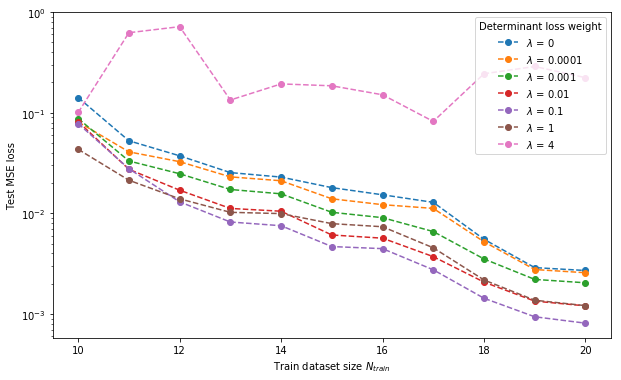
\includegraphics[width=\linewidth]{pnlty_det}
	\caption{Different weights $\lambda$ for $\mathcal{L}_{DET}$}
	\label{fig:pnlty_det}
\end{figure}


Looking at these results, we immediatly observe the method's robustness for different weights of the physical loss, since small weights in a range of at least two orders of magnitude, namely $\lambda \in [0.01, 1]$, lead to significantly improved performance. For smaller values of $\lambda$, the test error converges to the one of $\lambda= 0$, whereas values of $\lambda > 1$ lead to a heavy focus on satisfying the physical constraint and thus leads to poor results compared to smaller values and $\lambda=0$.\\
\indent Moreover, we can see that the choice $\lambda = 0.1$ consistently yields a smaller error on the test dataset. It is also important to note that the performance improvement is significant. For example, with only 20 training data points, the physically trained model achieves a Test MSE Loss of $8\times10^{-4}$, whereas the model trained solely on the MSE Loss achieves only a value of $2.7\times10^{-3}$, thus reducing the error by more than $70\%$. \\
\indent Interestingly, utilising the penalty method leads to higher performance even for larger train datasets. This can be seen in Figure \ref{fig:pnlty_det_large} in the appendix, displaying the results of an experiment we conducted on a wider range including up to 100 training data points.\\
We observe similar qualitative behaviour when applying the method for the 3D-rotation, as displayed in Figure \ref{fig:pnlty_det_dim3} in the Appendix.\\
\indent However, we are not only interested in the overall test performance, but also how realistic the predictions are. Figure \ref{fig:pnlty_det_analysis} shows the absolute difference of the determinant of the predicted rotation matrix and 1, the absolute difference of the norm of the predicted points and 1, and the test loss, all averaged across numerous points for each angle.\\
\begin{figure}[H]
	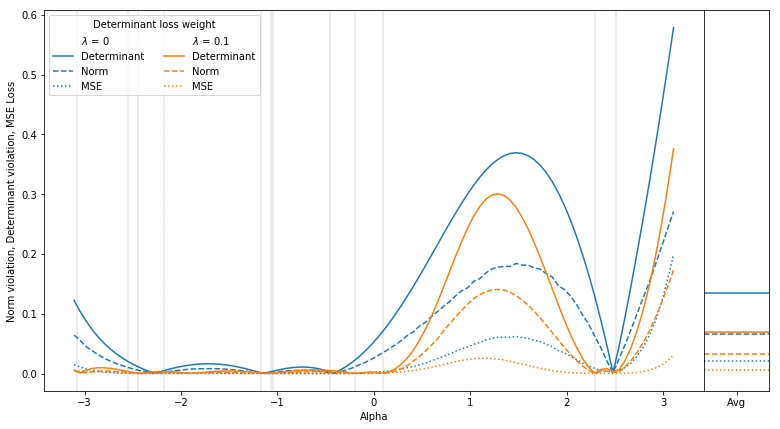
\includegraphics[width=\linewidth]{pnlty_det_analysis}
	\caption{Determinant and norm violations of predictions for $N_{train} = 12$. Gray vertical lines represent the angles of the training points.}
	\label{fig:pnlty_det_analysis}
\end{figure}
\indent First of all, we can see that the desired physical constraint is met perfectly at each training point, which already contributes to smaller overall errors in these regions. Even more important is the effect of the penalty method on predictions in areas where training data is sparse. An interesting region to analyse is the one for angles between $0.2$ and $2.2$, where not a single training data point exists. We can observe both smaller deviation of the determinant from one and smaller test error, meaning that the predictions are not only more realistic, but also closer to the true values.

\subsubsection{Increasing physical loss weight}
When analysing the version of the penalty method where we solve a series of minimisation problems with increasing weights $\lambda$ for $\mathcal{L}_{DET}$, we first have to discuss finding a good set of parameters. The parameters we need to determine for this method are the following:
\begin{itemize}
	\item Initial weight $\lambda_0 > 0$,
	\item Multiplier $\mu > 1$ which determines $\lambda_k = \mu^k\lambda_0$,
	\item Condition when to stop the current iteration,
	\item Number of iterations.
\end{itemize}
\begin{figure}[H]
	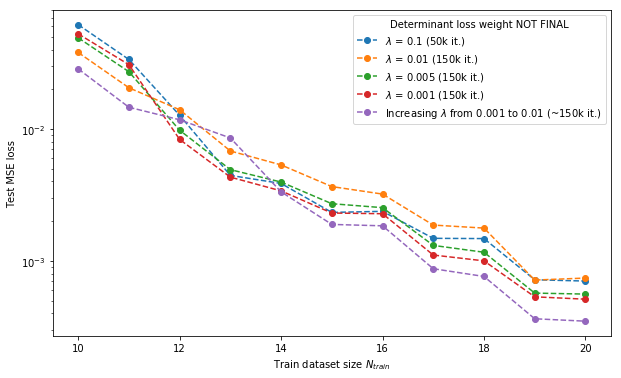
\includegraphics[width=\linewidth]{pnly_dyn}
	\caption{Different weights $\lambda$ for $\mathcal{L}_{DET}$ compared with dynamically increasing $\lambda$, averaged over 10 different training datasets.}
	\label{fig:pnly_dyn}
\end{figure}
In general, we can say that it is difficult to find a successful set of parameters, since we only have an intuition about the initial and last value of $\lambda$. We manually tried several different parameter sets, of which many led to much worse performance than the results shown above. However, we were able to increase performance with the following values: We set $\lambda_0 = 10^{-3}$, $\mu = 1.05$, use 50 iterations and stop the k-th iteration once the norm of the gradient is smaller than $0.95^{k} 10^{-3}$. With this, we get a last weight value of $\lambda_{50} \approx 10^{-2}$. However, since solving a series of minimisation problems with the chosen parameters involves approximately $150k$ iterations, we also compare the results with using the fixed method for $150k$ iterations for different values taken by $\lambda$ during the dynamic training process. The results are illustrated in Figure \ref{fig:pnly_dyn}. We can see that the dynamic version outperforms the fixed Penalty Method by a significant margin for most training dataset sizes. For example, for 20 data points, the former achieves an error of $3.5\times 10^{-4}$, whereas the best fixed version only reaches twice the error of $7\times 10^{-4}$. Unfortunately, the improvement is not consistent and for 13 data points, the dynamic version only achieves $8.5 \times 10^{-3}$, whereas even the fixed Penalty Method with only 50000 iterations already achieves with a value of $4.3 \times 10^{-3}$ almost half of this error.

As a summary, for the chosen parameters, the dynamic Penalty Method overall achieves higher performance than the fixed version. However, since it requires a multiple of the epochs needed by the fixed method and it is difficult to find a well performing set of parameters, we in general advise to use the simpler method using a fixed physical loss weight $\lambda$.

\subsection{Augmented Lagrangian Method}

We first apply the version which only computes a fixed number of epochs for each minimisation problem, and keep the weight $\lambda$ of the physical loss $\mathcal{L}_{DET}$ constant. Thus, it differs from the first version of the Penalty Method only in having the additional linear constraint violation term. Note that for ALM, this weight needs to be chosen significantly smaller than for the Penalty Method depending on the constraint violation, since the linear term is much higher relative to the squared constraint violation term for small violation values. Still, it is similarly difficult to find a good set of parameters as it is for the second version of the Penalty Method. We achieved reasonable performance computing 30 iterations with 5000 epochs each and a physical loss weight of $\lambda = 0.01$. The results are depicted in Figure \ref{fig:aug_lag} as "ALM fixed". In order to clearly extract the effect of incorporating ALM's core idea of including the linear constraint violation terms, we also include "ALM fixed (no linear)", which uses the same loss function, but omitting the linear terms. The results show that by using ALM with a good set of parameters, we can achieve even smaller error rates than the Penalty Method. For example, for 20 data points, the fixed ALM achieves an error of $3.9 \times 10^{-4}$, which is an improvement of $44\%$ compared to the error of $7 \times 10^{-4}$ of the Penalty Method, and also reduces the error by $24\%$ compared to its version which omits the linear term, which reaches an error of $5.1 \times 10^{-4} $\\
\indent However, the improvements are not very consistent in the range between 10 and 15 training data points. Further, we have to note that the method again needs $150k$ epochs in total compared to the $50k$ epochs of the fixed Penalty Method in order to achieve comparable results. An example of the training and test loss after each iteration when applying the fixed ALM is shown in Figure \ref{fig:alm_fixed_training} in the Appendix. Since the Lagrangian multiplier estimates can be negative, we included the negative linear loss for the determinant as well.
\begin{figure}[H]
	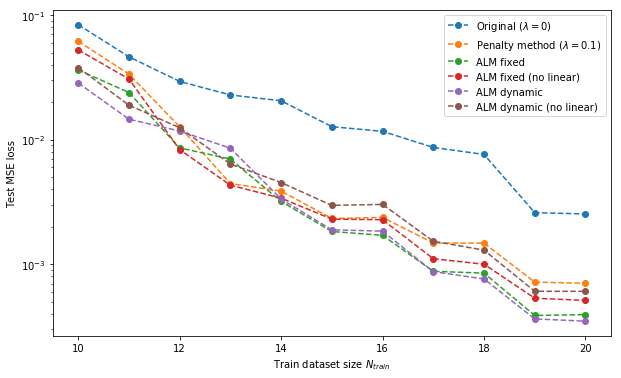
\includegraphics[width=\linewidth]{aug_lag}
	\caption{Comparison of ALM, Penalty Method and original training, averaged over 10 different random training datasets.}
	\label{fig:aug_lag}
\end{figure}
Furthermore, Figure \ref{fig:aug_lag} depicts the results of applying the second version of ALM, again including the comparison with the same computation without the linear term in the loss function. As described in section \ref{exp:alm}, we need to determine even more parameters than we do for the first version of ALM or the Penalty Method. This makes it especially difficult to find good parameters, and we need to mention that throughout the process of finding a good parameter set, we have tried many values that led to significantly worse performance than the original model which does not incorporate any physical constraints at all. To get reasonable results, we chose the following parameters: To begin with, we set $\lambda_{0} = 10^{-3}$ and increased it by a factor of $1.05$ after each iteration. By computing 50 iterations, $\lambda$ increases by approximately one order of magnitude. In order to make use of the proposed idea of setting the gradient threshold to a minimum of a fixed value and one dependent on the constraint violation, we set $\gamma_k = 0.95^k\,10^{-1}$ and $\epsilon_k = 0.95^k\,10^{-3}$. These values were chosen after analysing the constraint violation values during training and set such that $\epsilon_k$ and $\gamma_k ||c(x_k)||$ have approximately the same order of magnitude. The achieved results using these parameters are similiar to the fixed ALM results, and again achieve smaller error rates than the corresponding training omitting the linear term. For 20 training data points, it achieves an error of $3.5\times 10^{-4}$, which is close to the $3.9 \times 10^{-4}$ achieved by the fixed ALM. Overall, this is an improvement of $86\%$ compared to the original model which does not incorporate phyiscal constraints and thus only reaches an error of $2.5\times 10^{-3}$. However, also this version of ALM does not perform consistently better than the Penalty Method. Furthermore, it needs at least $150k$ and up to $300k$ epochs to achieve these results. Detailed numbers and statistics on the explained experiment are given in the Appendix (Table \ref{table_stats_10} - \ref{table_stats_20}).\\
\indent To understand the impact of ALM on how well the predictions align with the physical constraints, Figure \ref{fig:alm_det_analysis} depicts the absolute difference of the prediction norms and one, the absolute difference of the determinant of the predicted rotation matrix and one, and the corresponding MSE Loss. Note that results vary and Figure \ref{fig:alm_det_analysis} only depicts the values for 12 training data points and a single seed used to generate the training dataset.

\begin{figure}[H]
	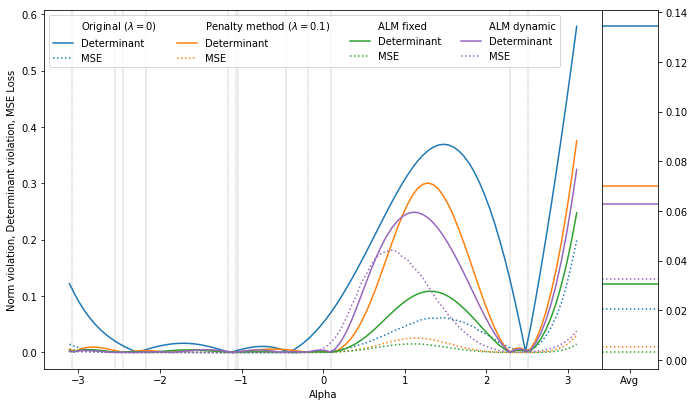
\includegraphics[width=\linewidth]{alm_det_analysis}
	\caption{Determinant and norm violations of predictions for $N_{train} = 12$. Gray vertical lines represent the angles of the training points.}
	\label{fig:alm_det_analysis}
\end{figure}

As expected knowing the statistical performance of the methods, the deviations from the physical constraints are significantly smaller when we apply one of the proposed methods compared to the original training. Similar to the Penalty Method, both versions of the Augmented Lagragian Method lead to no constraint violations at points where training data is present. While the fixed ALM in this case generalises the physical constraints significantly better than the Penalty Method, the dynamic version achieves only comparable results. Despite, an interesting observation is the high MSE Loss average of the dynamic ALM, which exceeds with a value of 0.033 the error of all other methods significantly. Even the original model achieves an overall average of the MSE Loss of only 0.021. However, this is only due to the performance in the range of angles between 0 and 2, for the extrapolation of angles higher than 2.5, it performs much better than the original model. This is the case even though the determinant in the difficult region is much closer to one than the determinant of the prediction of the original model. This indicates that the ALM focused too much on learning the determinant constraint, since it is able to generalise the determinant constraint only at cost of the performance of the predictions for this specific case.\\
\indent Furthermore, we want to point out that finding a good condition when to stop the training process is difficult. The test performance throughout the training process for different randomly generated training datasets is depcited in Figure \ref{fig:test_training}. When comparing the performance of the Penalty Method (left) with the Dynamic ALM (right), we can instantly see much higher deviations when using the latter method. For example, the test performance colored in blue reaches a test MSE Loss of less than $0.7\times 10^{-4}$, but only achieves an error of more than $3\times 10^{-2}$ when training has ended. In contrast, most of the test errors of using the Penalty Method converge and following epochs only lead to slight overfitting. This in turn indicates the high potential of ALM as well. As we can see, the best performance achieved often exceeds the final performance significantly. More sophisticated methods used to determine the hyperparameters of ALM  might therefore lead to much higher improvements compared to what we achieve with the current parameters. For three dimensions, we were not able to find a set of parameters leading to any improvements compared to the original model.
\begin{figure}
	\centering
	\begin{subfigure}{.5\textwidth}
		\centering
		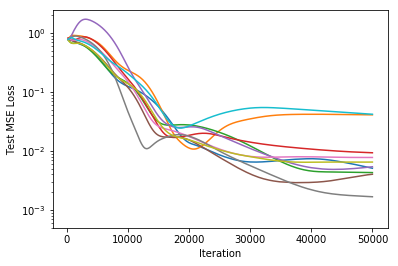
\includegraphics[width=\linewidth]{rand_test_pnlty}
		\caption{Penalty method with $\lambda = 0.1$}
	\end{subfigure}%
	\begin{subfigure}{.5\textwidth}
		\centering
		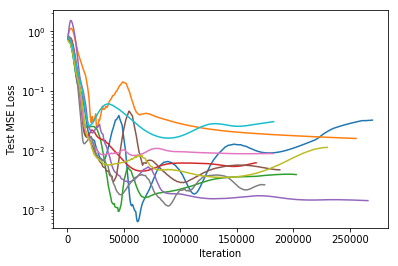
\includegraphics[width=\linewidth]{rand_test_alm_dyn}
		\caption{Dynamic ALM}
	\end{subfigure}
	\caption{Test error throughout the training process, each color represents a different training dataset.}
	\label{fig:test_training}
\end{figure}






\subsection{Failed experiments}

\subsubsection{Norm physical loss}
As we did for the physical constraint \ref{eq:constraint_det} of the determinant being equal to one, we also tried to incorporate the constraint \ref{eq:constraint_norm}, which says that the norm of the predicted point is supposed to be one. In contrast to what we expected and what we achieved incorporating the determinant constraint, we were not able to improve the performance of our model using the Penalty Method on the violation of the norm constraint. The results for different weights for $\mathcal{L}_{NORM}$ in the training loss for two and three dimensions are shown in Figure \ref{fig:pnlny_norm} in the Appendix.

\subsubsection{Physical Projection}
As explained in section \ref{sec:phys_proj}, we also tested an approach we call Physical Projection. We first applied it to the determinant constraint, thus scaling every predicted matrix with positive determinant according to Equation \ref{eq:norm_det}. Note that we detach the calculated scaling factor in order to not influence the gradient. Unfortunately, training using this procedure does not converge, an example is shown in Figure \ref{fig:normed_det_example} in the appendix.\\
\indent When applying the Physical Projection to the norm constraint, we again detach the calculated norm and only determine training loss and its gradient on the error between the normed prediction and the true point. As we can see in Figure \ref{fig:normed_pred} in the appendix, this approach does not improve the performance for either two or three dimensions. When further investigating the reason for this behaviour, we noticed that the norm of the predictions before scaling differs for regions that lack training data between them. The illustration in Figure \ref{fig:normed_pred_example} shows this behaviour well: For $-\pi < \alpha < 0.5$, the determinant of the predicted rotation matrix is only $\frac{1}{10}$ of the predicted determinant for $2 < \alpha < 3$. Even though predictions after the projection align with the physical constraints, it adds complexity to the problem, since the model can not make use of the rule that the determinant or norm is consistent accross all angles.







\clearpage



% !TEX root = ../main.tex
\label{section:discussion}
\section{Discussion}

To conclude this thesis, we summarise the main results of incorporating physical constraints into deep learning models. First of all, we empirically showed that the knowledge about scientific principles, when correctly maken use of, can improve overall performance significantly and also helps to make predictions more realistic. However, since this was only possible using the determinant and not with the norm constraint, we saw that there is no such guarantee for all physical constraints. One might reason that principles that reveal more complicated underlying structures of the process such as the determinant of a rotation matrix lead to higher improvements, since they are otherwise hard to learn. This is especially true when only few training data is available. We were also able to show that the proposed methods lead to smaller training error in regions where training data is sparse.\\
\indent When comparing the Penalty Method to the Augmented Lagrangian Method, it is important to note that even though ALM leads to higher performance and showed high potential when terminating training at the right time, there are currently no known methods to the author that estimate hyperparameters well. Since the Penalty Method is easy to understand   and to implement, robust to the physical loss weight and requires less epochs, we advice to first apply this method and only search for good ALM hyperparameters once applying the Penalty Method has shown improvements. Furthermore, we were not able to yield improvements using the method of Physical Projections on any constraint.\\
\indent For future studies, we suggest to explore ways to find better parameters for ALM leading to more consistent results and requiring less training iterations. Furthermore, one might train the model on simulated unsupervised data to align its predictions with physical constraints in regions where no training data exists.









\clearpage




% ---------------------------------------------------------------------------
%
%Introduction and Background Theory
%
% ---------------------------------------------------------------------------
\cleardoubleemptypage
\label{part:introAndBackgroundTheory}
%% !TEX root = ../main.tex
\section{Introduction}
\label{chapter:Introduction}
	This document has been created in order to show you some of the capabilities 
of \LaTeX.  A great resource for an introduction to \LaTeX\xspace is Tobias
Oetiker's ''The Not So Short Introduction to \LaTeXe'' \cite{latex}.  Please
page through that document
before starting with your thesis.
Oh, and let's use the mysterious word \gls{computer} here to give the glossary
a reason to appear.
A third useful option to reference stuff besides citing or glossarying (?) 
is using footnotes. Just like
this\footnote{Properly formatted clickable URL: \url{https://www.tum.de/}}
one.
And: lists! Lists with bullet points are amazing. I mean, just look at this:
\begin{itemize}
	\item list
	\item all 
	\item the 
	\item things!
\end{itemize}
% use enumerate for numbers instead of points: 
% https://en.wikibooks.org/wiki/LaTeX/List_Structures#List_structures
\par
Anyways your introduction goes here.


Below a few \LaTeX examples are included for beginners
\comment{You can also put comments in the margins for you or your advisor}
\begin{figure}[ht]
  \centering
  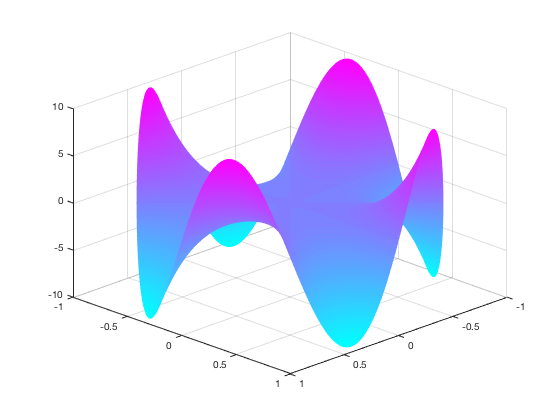
\includegraphics[width=5cm]{images/swing_function_plot.png}
  \caption{$u(x)$}%{Numerically solved solution}
  \label{fig:swingPlot}
\end{figure}


Equations can also be labeled
\begin{equation}
	\pi = \mathrm{e}^{i\cdot\phi}
	\label{eq:equation1}
\end{equation}


And later referenced. Even in subfigures.
\begin{figure}[!htb]
  \centering
  \begin{subfigure}[b]{0.3\textwidth}
    \centering
  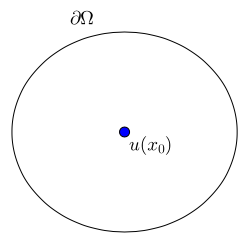
\includegraphics[width=\textwidth]{images/CircCenter}
  \caption{Equation \ref{eq:equation1}}\label{fig:circcenter}
\end{subfigure}
\hfill
  \begin{subfigure}[b]{0.3\textwidth}
    \centering
  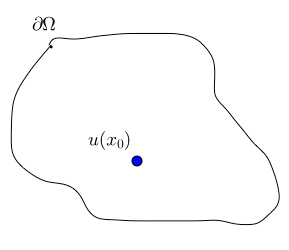
\includegraphics[width=\textwidth]{images/GeneralOffset}
  \label{fig:generaloffset}
  \caption{Equation \ref{eq:equation1}}
\end{subfigure}
\end{figure}
\subsection{Including code}

Code can be using the package
\href{https://www.sharelatex.com/learn/Code\_Highlighting\_with\_minted}{Minted}.

An exaple of which of can be found below (see Source Code \ref{lst:nice_listing})
\begin{listing}
	%the language syntax can be declared here.
	\begin{minted}{python} 
	import numpy as np
	
	def incmatrix(genl1,genl2):
	    m = len(genl1)
	    n = len(genl2)
	    M = None #to become the incidence matrix
	    VT = np.zeros((n*m,1), int)  #dummy variable
	
	    #compute the bitwise xor matrix
	    M1 = bitxormatrix(genl1)
	    M2 = np.triu(bitxormatrix(genl2),1)
	
	    for i in range(m-1):
	        for j in range(i+1, m):
	            [r,c] = np.where(M2 == M1[i,j])
	            for k in range(len(r)):
	                VT[(i)*n + r[k]] = 1;
	                VT[(i)*n + c[k]] = 1;
	                VT[(j)*n + r[k]] = 1;
	                VT[(j)*n + c[k]] = 1;
	
	                if M is None:
	                    M = np.copy(VT)
	                else:
	                    M = np.concatenate((M, VT), 1)
	
	                VT = np.zeros((n*m,1), int)
	
	    return M
	\end{minted}

  \caption{My nice listing}
  \label{lst:nice_listing}
\end{listing}


%
%% ---------------------------------------------------------------------------
%%
%% Thesis content: What did you do?
%%
%%% ---------------------------------------------------------------------------


%% ---------------------------------------------------------------------------
%%
%% Results and Conclusion
%%
%% ---------------------------------------------------------------------------



% ---------------------------------------------------------------------------
%
% Appendix
%
% ---------------------------------------------------------------------------
\part*{Appendix}
\addcontentsline{toc}{part}{Appendix}

\appendix %---------------------------------------

% !TEX root = ../main.tex

\label{appendix}

\begin{proof}[Proof that the determinant of the rotation matrix in two dimensions equals one \eqref{eq:constraint_det}\\]$\,$\\
	Let $\alpha \in [-\pi, \pi]$ be an arbitrary rotation angle. Then we have
	\begin{equation}
		\label{proof:det_one}
		\begin{aligned}
		 \det (R_{2D}(\alpha)) &= \det \begin{pmatrix} \cos(\alpha) & -\sin(\alpha) \\\sin(\alpha) & \cos(\alpha) \end{pmatrix} \\
		&= \cos(\alpha)\cos(\alpha) - \sin(\alpha)(- \sin(\alpha))\\
		&= \cos(\alpha)^2 + \sin(\alpha)^2\\
		&= 1
		\end{aligned}
	\end{equation}
\end{proof}

\begin{proof}[Proof that the determinant of the rotation matrix in three dimensions equals one \eqref{eq:constraint_det}\\]$\,$\\
	Let $\alpha \in [-\pi, \pi]^2$ be an arbitrary rotation angle. Then we have
	\begin{equation}
	\label{proof:det_one_dim3}
	\begin{aligned}
	\det (R_{3D}(x, \vec{\alpha})) &= \det(R_{y}(\alpha_2) R_{z}(\alpha_1)) \\
	&= \det \left( \begin{pmatrix} \cos(\alpha_2) & -\sin(\alpha_2) & 0\\\sin(\alpha_2) & \cos(\alpha_2) & 0\\ 0 & 0 & 1\end{pmatrix} \begin{pmatrix} \cos(\alpha_1) & 0 & -\sin(\alpha_1)\\ 0 & 1 & 0\\\sin(\alpha_1) & 0 & \cos(\alpha_1)\end{pmatrix} \right)\\
	&= \det \begin{pmatrix} \cos(\alpha_2) & -\sin(\alpha_2) & 0\\\sin(\alpha_2) & \cos(\alpha_2) & 0\\ 0 & 0 & 1\end{pmatrix} \cdot \det \begin{pmatrix} \cos(\alpha_1) & 0 & -\sin(\alpha_1)\\ 0 & 1 & 0\\\sin(\alpha_1) & 0 & \cos(\alpha_1)\end{pmatrix}\\
	&= (\cos(\alpha_2)^2 + \sin(\alpha_2)^2) \cdot (\cos(\alpha_1)^2 + \sin(\alpha_1)^2)\\
	&= 1
	\end{aligned}
	\end{equation}
\end{proof}

\begin{proof}[Proof for the norm preservation by the rotation in two dimensions \eqref{eq:constraint_norm}\\]$\,$\\
	Let $p = \begin{pmatrix}x \\y \\\end{pmatrix}$ be any input vector with $x, y \in \mathbb{R}$ and $\alpha \in [-\pi, \pi]$ an arbitrary rotation angle. Since $||\cdot|| \geq 0$, it is sufficient to show that $||rot_{2D}(p, \vec{\alpha})||_2^2 = ||p||_2^2$.
	\begin{equation}
	\label{proof:norm_preservation}
	\begin{aligned}
	||rot_{2D}(p, \alpha)||_2 &= \left\Vert \begin{pmatrix} \cos(\alpha) & -\sin(\alpha) \\\sin(\alpha) & \cos(\alpha) \end{pmatrix} \begin{pmatrix}x \\y \\\end{pmatrix} \right\Vert_2^2 \\
	&= (\cos(\alpha)x - \sin(\alpha)y)^2 + (\sin(\alpha)x + \cos(\alpha)y)^2\\
	&= \cos(\alpha)^2x^2 -2\cos(\alpha)x\sin(\alpha)y \sin(\alpha)^2y^2 + \sin(\alpha)^2y^2\\ &\,\,\,\,\,\,\,\,\,+ \sin(\alpha)^2x^2 + 2\sin(\alpha)x\cos(\alpha)y + \cos(\alpha)^2y^2\\
	&= (\cos(\alpha)^2 + \sin(\alpha)^2)x^2 + (\sin(\alpha)^2 + \cos(\alpha)^2)y^2\\
	&= x^2 + y^2\\
	&= ||p||_2^2
	\end{aligned}
	\end{equation}
\end{proof}

\begin{proof}[Proof for the norm preservation by the rotation in three dimensions \eqref{eq:constraint_norm}\\]$\,$\\
	Let $p = \begin{pmatrix}x \\y \\z \\\end{pmatrix}$ be any input vector with $x, y, z \in \mathbb{R}$ and $\alpha \in [-\pi, \pi]^2$ an arbitrary rotation angle. Since $||\cdot|| \geq 0$, it is sufficient to show that $||rot_{3D}(p, \vec{\alpha})||_2^2 = ||p||_2^2$.
	\begin{equation}
	\label{proof:norm_preservation_dim3}
	\begin{aligned}
	||rot_{3D}(p, \vec{\alpha})||_2^2 &= \left\Vert R_{y}(\alpha_2) R_{z}(\alpha_1) p \right\Vert_2^2 \\
	&= \left\Vert \begin{pmatrix} \cos(\alpha_2) & -\sin(\alpha_2) & 0\\\sin(\alpha_2) & \cos(\alpha_2) & 0\\ 0 & 0 & 1\end{pmatrix} \begin{pmatrix} \cos(\alpha_1) & 0 & -\sin(\alpha_1)\\ 0 & 1 & 0\\\sin(\alpha_1) & 0 & \cos(\alpha_1)\end{pmatrix} \begin{pmatrix}x \\y \\z \\\end{pmatrix} \right\Vert_2^2 \\
	&= \left\Vert \begin{pmatrix} \cos(\alpha_2) & -\sin(\alpha_2) & 0\\\sin(\alpha_2) & \cos(\alpha_2) & 0\\ 0 & 0 & 1\end{pmatrix} \begin{pmatrix}\cos(\alpha_1)x - \sin(\alpha_1)z \\y \\\sin(\alpha_1)x + \cos(\alpha_1)z \\\end{pmatrix} \right\Vert_2^2 \\
	&= \left\Vert \begin{pmatrix}\cos(\alpha_2)(\cos(\alpha_1)x - \sin(\alpha_1)z) - \sin(\alpha_2)y \\
	\sin(\alpha_2)(\cos(\alpha_1)x - \sin(\alpha_1)z) + \cos(\alpha_2)y \\
	\sin(\alpha_1)x + \cos(\alpha_1)z \\\end{pmatrix} \right\Vert_2^2 \\
	&= (\cos(\alpha_2)^2 + \sin(\alpha_2)^2)(\cos(\alpha_1)x - \sin(\alpha_1)z)^2 + \sin(\alpha_2)^2y^2 + \cos(\alpha_2)^2y^2 \\ 
	&\,\,\,\,\,\,\,\,\,+ \sin(\alpha_1)^2x^2 + 2\sin(\alpha_1)x\cos(\alpha_1)z + \cos(\alpha_1)^2z^2\\
	&= \cos(\alpha_1)^2x^2 + \sin(\alpha_1)^2z^2 + y^2 + \sin(\alpha_1)^2x^2 + \cos(\alpha_1)^2z^2\\
	&= x^2 + y^2 + z^2\\
	&= ||p||_2^2
	\end{aligned}
	\end{equation}
\end{proof}

\begin{figure}[H]
	\centering
	\begin{subfigure}{.5\textwidth}
		\centering
		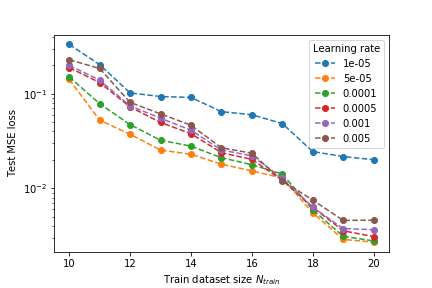
\includegraphics[width=\linewidth]{lr_dim2_m3}
		\caption{2 dimensions}
	\end{subfigure}%
	\begin{subfigure}{.5\textwidth}
		\centering
		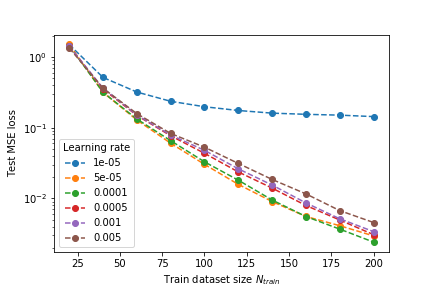
\includegraphics[width=\linewidth]{lr_dim3_m3}
		\caption{3 dimensions}
	\end{subfigure}
	\caption{Comparison of learning rates for Model 3}
	\label{fig:comp_lr_m3}
\end{figure}

\begin{figure}[H]
	\centering
	\begin{subfigure}{.5\textwidth}
		\centering
		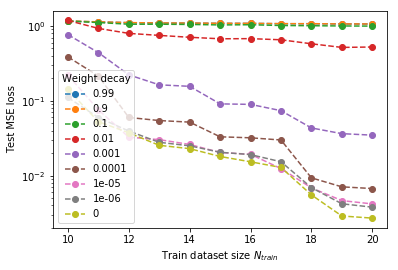
\includegraphics[width=\linewidth]{reg_weights}
		\caption{2 dimensions}
	\end{subfigure}%
	\begin{subfigure}{.5\textwidth}
		\centering
		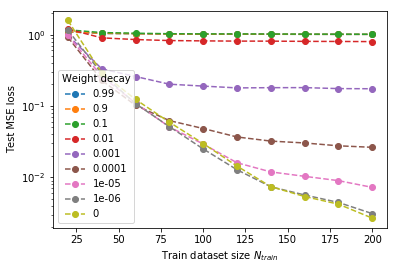
\includegraphics[width=\linewidth]{reg_weights_dim3}
		\caption{3 dimensions}
	\end{subfigure}
	\caption{L2-Regularisation weights on Model 3}
	\label{fig:reg_weights}
\end{figure}


\begin{figure}[H]
	\centering
	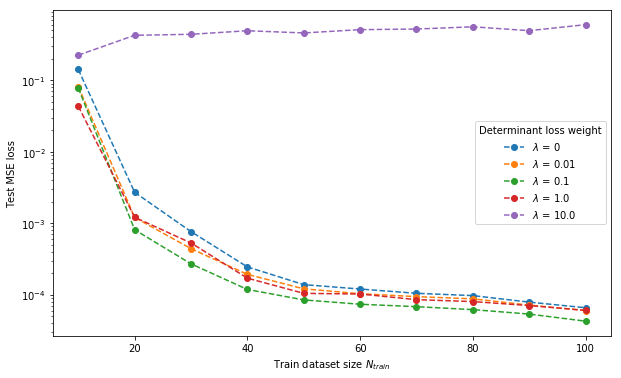
\includegraphics[width=0.7\linewidth]{pnlty_det_large}
	\caption{Different weights $\lambda$ for $L_{DET}$ in 2D}
	\label{fig:pnlty_det_large}
\end{figure}

\begin{figure}[H]
	\centering
	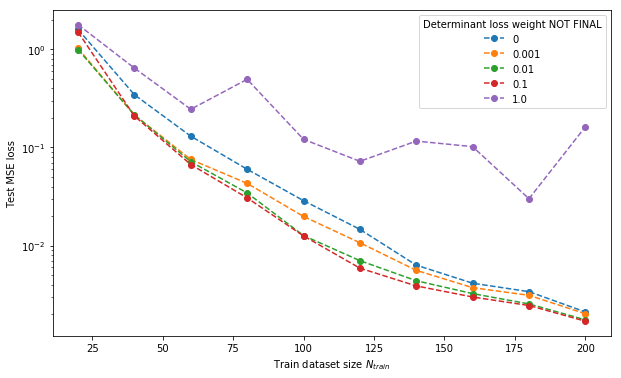
\includegraphics[width=0.7\linewidth]{pnlty_det_dim3}
	\caption{Different weights $\lambda$ for $L_{DET}$ in 3D}
	\label{fig:pnlty_det_dim3}
\end{figure}

\begin{figure}[H]
\centering
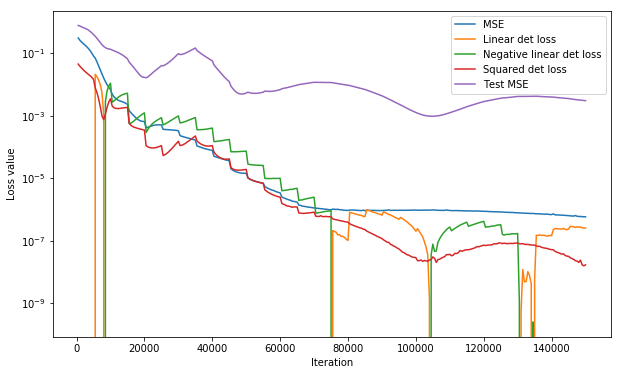
\includegraphics[width=0.7\linewidth]{alm_fixed_training}
\caption{Loss values during training of the fixed ALM in 2D for $N_{train} = 12$ and a single random seed.}
\label{fig:alm_fixed_training}
\end{figure}

\begin{table}[H]
\centering
\resizebox{\columnwidth}{!}{%
\begin{tabular}{lrrrrrrrr}
	\midrule
	{} &  count &      mean &       std &       min &       25\% &       50\% &       75\% &       max \\ \midrule
	Original ($\lambda = 0$)         &   10.0 &  0.083873 &  0.084808 &  0.017509 &  0.025126 &  0.051635 &  0.102614 &  0.258126 \\ \midrule
	Penalty method ($\lambda = 0.1$) &   10.0 &  0.061773 &  0.089446 &  0.002449 &  0.006697 &  0.018631 &  0.095302 &  0.280234 \\ \midrule
	ALM fixed                        &   10.0 &  0.036335 &  0.041466 &  0.001796 &  0.007078 &  0.014448 &  0.054447 &  0.119299 \\ \midrule
	ALM dynamic                      &   10.0 &  0.028551 &  0.026700 &  0.005898 &  0.009325 &  0.017179 &  0.041241 &  0.079159 \\ \midrule
\end{tabular}
}
\caption{Test MSE Loss statistics for 10 random training sets and $N_{train} = 10$}
\label{table_stats_10}
\end{table}

\begin{table}[H]
	\centering
	\resizebox{\columnwidth}{!}{%
		\begin{tabular}{lrrrrrrrr}
			{} &  count &      mean &       std &       min &       25\% &       50\% &       75\% &       max \\ \midrule
			Original ($\lambda = 0$)         &   10.0 &  0.012718 &  0.009706 &  0.000652 &  0.006690 &  0.010347 &  0.014473 &  0.032356 \\ \midrule
			Penalty method ($\lambda = 0.1$) &   10.0 &  0.002330 &  0.001577 &  0.000174 &  0.001137 &  0.002370 &  0.003468 &  0.004632 \\ \midrule
			ALM fixed                        &   10.0 &  0.001832 &  0.001621 &  0.000128 &  0.000656 &  0.001172 &  0.002869 &  0.004497 \\ \midrule
			ALM dynamic                      &   10.0 &  0.001889 &  0.001693 &  0.000094 &  0.000804 &  0.001271 &  0.002364 &  0.005209 \\ \midrule
		\end{tabular}
	}
	\caption{Test MSE Loss statistics for 10 random training sets and $N_{train} = 15$}
	\label{table_stats_15}
\end{table}

\begin{table}[H]
	\centering
	\resizebox{\columnwidth}{!}{%
		\begin{tabular}{lrrrrrrrr}
			{} &  count &      mean &       std &       min &       25\% &       50\% &       75\% &       max \\ \midrule
			Original ($\lambda = 0$)         &   10.0 &  0.002534 &  0.002381 &  0.000539 &  0.000931 &  0.001674 &  0.003141 &  0.007491 \\ \midrule
			Penalty method ($\lambda = 0.1$) &   10.0 &  0.000703 &  0.000487 &  0.000154 &  0.000260 &  0.000686 &  0.000999 &  0.001665 \\ \midrule
			ALM fixed                        &   10.0 &  0.000394 &  0.000422 &  0.000072 &  0.000140 &  0.000174 &  0.000511 &  0.001419 \\ \midrule
			ALM dynamic                      &   10.0 &  0.000349 &  0.000332 &  0.000016 &  0.000072 &  0.000211 &  0.000564 &  0.000922 \\ \midrule
		\end{tabular}
	}
	\caption{Test MSE Loss statistics for 10 random training sets and $N_{train} = 20$}
	\label{table_stats_20}
\end{table}


\begin{figure}[H]
	\centering
	\begin{subfigure}{.5\textwidth}
		\centering
		\includegraphics[width=\linewidth]{lag_mu}
		\caption{Physical loss weight $\mu$}
	\end{subfigure}%
	\begin{subfigure}{.5\textwidth}
		\centering
		\includegraphics[width=\linewidth]{lag_est}
		\caption{Lagrangian multiplier estimates $\lambda$}
	\end{subfigure}
	\caption{Values for the physical loss weight $\mu$ and the Lagrangian multiplier estimates $\lambda$ when training using the dynamic ALM with $N_{train} = 12$.}
	\label{fig:mu_lambda_alm_dyn}
\end{figure}


\begin{figure}[H]
	\centering
	\begin{subfigure}{.5\textwidth}
		\centering
		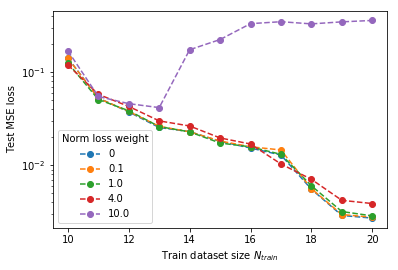
\includegraphics[width=\linewidth]{pnlty_norm}
		\caption{2 dimensions}
	\end{subfigure}%
	\begin{subfigure}{.5\textwidth}
		\centering
		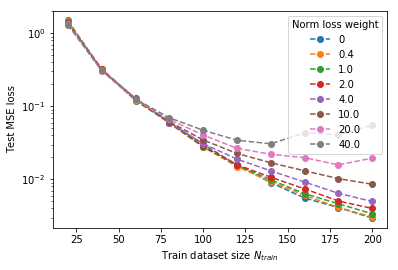
\includegraphics[width=\linewidth]{pnlty_norm_3}
		\caption{3 dimensions}
	\end{subfigure}
	\caption{Penalty Method on the Norm constraint}
	\label{fig:pnlny_norm}
\end{figure}


\begin{figure}[H]
	\centering
	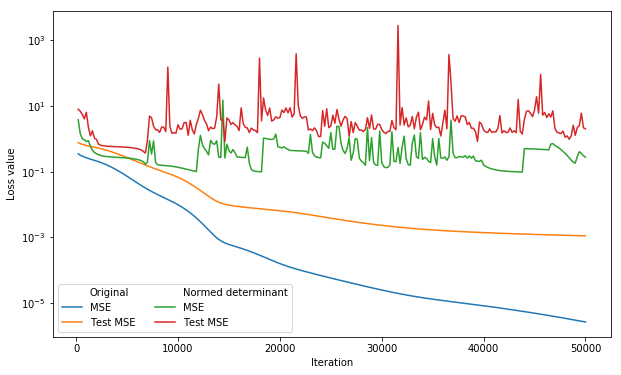
\includegraphics[width=0.7\linewidth]{normed_det_example}
	\caption{Training for 2 dimensions and $N_{train} = 20$ using the original training and the Physical projection on the determinant with the same training dataset.}
	\label{fig:normed_det_example}
\end{figure}

\begin{figure}[H]
	\centering
	\begin{subfigure}{.5\textwidth}
		\centering
		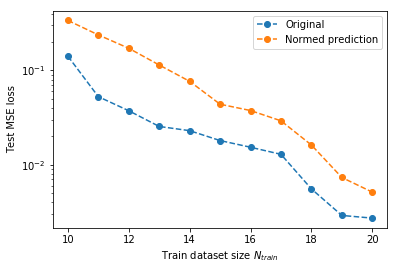
\includegraphics[width=\linewidth]{normed_pred}
		\caption{2 dimensions}
	\end{subfigure}%
	\begin{subfigure}{.5\textwidth}
		\centering
		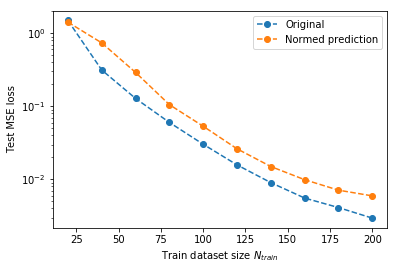
\includegraphics[width=\linewidth]{normed_pred_3}
		\caption{3 dimensions}
	\end{subfigure}
	\caption{Physical projection on the norm of the prediction}
	\label{fig:normed_pred}
\end{figure}

\begin{figure}[H]
	\centering
	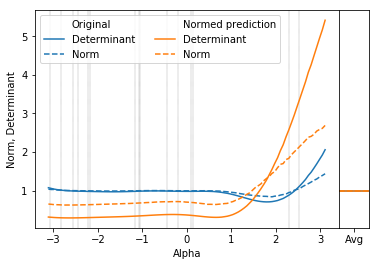
\includegraphics[width=0.7\linewidth]{normed_pred_example}
	\caption{Analysis of the predictions of a model trained using Physical Projection on the norm compared to the original model. All determinants and norms are scaled such that their mean is equal to one.}
	\label{fig:normed_pred_example}
\end{figure}


\clearpage



 \printglossaries

 \addcontentsline{toc}{chapter}{Bibliography}
 \bibliography{bibliography/literature}

\end{document}
